%%%%%%%%%%%%%%%%%%%%%%%%%%%%%%%%%%%%%%%%%
% Stylish Article
% LaTeX Template
% Version 2.0 (13/4/14)
%
% This template has been downloaded from:
% http://www.LaTeXTemplates.com
%
% Original author:
% Mathias Legrand (legrand.mathias@gmail.com)
%
% License:
% CC BY-NC-SA 3.0 (http://creativecommons.org/licenses/by-nc-sa/3.0/)
%
%%%%%%%%%%%%%%%%%%%%%%%%%%%%%%%%%%%%%%%%%

%----------------------------------------------------------------------------------------
%	PACKAGES AND OTHER DOCUMENT CONFIGURATIONS
%----------------------------------------------------------------------------------------

\documentclass[fleqn,10pt]{SelfArx} % Document font size and equations flushed left

\usepackage{lipsum} % Required to insert dummy text. To be removed otherwise

%----------------------------------------------------------------------------------------
%	COLUMNS
%----------------------------------------------------------------------------------------

\setlength{\columnsep}{0.55cm} % Distance between the two columns of text
\setlength{\fboxrule}{0.75pt} % Width of the border around the abstract

%----------------------------------------------------------------------------------------
%	COLORS
%----------------------------------------------------------------------------------------

\definecolor{color1}{RGB}{0,0,90} % Color of the article title and sections
\definecolor{color2}{RGB}{0,20,20} % Color of the boxes behind the abstract and headings

%----------------------------------------------------------------------------------------
%	HYPERLINKS
%----------------------------------------------------------------------------------------

\usepackage{hyperref} % Required for hyperlinks
\hypersetup{hidelinks,colorlinks,breaklinks=true,urlcolor=color2,citecolor=color1,linkcolor=color1,bookmarksopen=false,pdftitle={Title},pdfauthor={Author}}

%----------------------------------------------------------------------------------------
%   MANUAL CONFIGURATION
%----------------------------------------------------------------------------------------

\graphicspath{{Images/}{Graphics/}}

\usepackage{todonotes}
\usepackage[author={Alexey Sofiev}]{pdfcomment}

\usepackage{algorithm}
\usepackage[noend]{algpseudocode}


%----------------------------------------------------------------------------------------
%   TABLE
%----------------------------------------------------------------------------------------

%
%\usepackage{xcolor}
%\usepackage{dcolumn}
%\usepackage{tabu}

\usepackage{tabulary,hhline}% http://ctan.org/pkg/{tabularx,hhline}

%----------------------------------------------------------------------------------------
%	ARTICLE INFORMATION
%----------------------------------------------------------------------------------------

%\JournalInfo{Journal, Vol. XXI, No. 1, 1-5, 2013} % Journal information
%\Archive{Additional note} % Additional notes (e.g. copyright, DOI, review/research article)
\JournalInfo{Labraselostus, Versio 1.2, 2015-2016} % Journal information
\Archive{Syventävä aineopintojen laboratoriotyö} % Additional notes (e.g. copyright, DOI, review/research article)



\PaperTitle{Monte Carlo study of a X-ray examination, the basis and the effects of the external radiation shields} % Article title

\Authors{Alexey Sofiev\textsuperscript{1}*, Anna Kelaranta\textsuperscript{2}, Mika Kortesniemi\textsuperscript{2}} % Authors
%\affiliation{\textsuperscript{1}\textit{Department of Biology, University of Examples, London, United Kingdom}} % Author affiliation
%\affiliation{\textsuperscript{2}\textit{Department of Chemistry, University of Examples, London, United Kingdom}} 
\affiliation{\textsuperscript{1}\textit{Tekijä}} % Author affiliation
\affiliation{\textsuperscript{2}\textit{Superviser}} 
% Author affiliation
%\affiliation{*\textbf{Corresponding author}: john@smith.com} % Corresponding author

\Keywords{BodyPhantom --- Eunice --- ImpactMC --- Dose map} % Keywords - if you don't want any simply remove all the text between the curly brackets
\newcommand{\keywordname}{Keywords} % Defines the keywords heading name

%----------------------------------------------------------------------------------------
%	ABSTRACT
%----------------------------------------------------------------------------------------

%\Abstract{\lipsum[1]~}
\Abstract{
Syventävä aineopintojen labra. Eunice-phantomi, annoslaskennan simulointi etc

~}


%----------------------------------------------------------------------------------------




%%%%% AS, adding image fixing.
%%%\usepackage{blindtext}
%%%\usepackage{graphicx}
%%%\usepackage{tcolorbox}
%%%
%%%
%%%\let\StandardIncludeGraphics\includegraphics%
%%%\renewcommand{\includegraphics}[2][]{%
%%%\IfFileExists{#2.eps}{%
%%%  \StandardIncludeGraphics[#1]{#2}%
%%%}{%
%%% \IfFileExists{#2.pdf}{%
%%%  \StandardIncludeGraphics[#1]{#2}%
%%%  }{ % No, no .pdf, try *.jpg 
%%%   \IfFileExists{#2.jpg}{%
%%%    \StandardIncludeGraphics[#1]{#2}%
%%%    }{
%%%      \IfFileExists{#2.png}{%
%%%      \StandardIncludeGraphics[#1]{#2}%
%%%      }{%
%%%      \begin{tcolorbox}[width=6cm,height=4cm,arc=0mm,auto outer arc]
%%%      \end{tcolorbox}
%%%     }
%%%   }
%%% }
%%%}% 
%%%%
%%%}% End of command
%----------------------------------------------------------------------------------------

\begin{document}

\flushbottom % Makes all text pages the same height

\maketitle % Print the title and abstract box

\tableofcontents % Print the contents section

\thispagestyle{empty} % Removes page numbering from the first page

%----------------------------------------------------------------------------------------
%	ARTICLE CONTENTS
%----------------------------------------------------------------------------------------

\section*{Introduction} % The \section*{} command stops section numbering

\addcontentsline{toc}{section}{Introduction} % Adds this section to the table of contents

%\vfill{}
%\vspace{5cm}

The radiological examination provides valuable information about the health of the patient and plays an important role in helping a doctor to make an accurate diagnosis. However, such an examination exposes the patient to the radiation, thus the benefit of the examination and the possible harm of the radiation dose must be cooperatively taken into account at a planning stage. 

It has been shown, that the most common and cost-effective examination in conventional radiography is the radiological examination. (Helasvuo 2013, Speets et al. 2006, Veldkamp et al. 2009, McAdams et al, 2006). Still, the effects of the external shields to reduce the dose are yet to be studied. One of possible approaches for such investigation is simulating the situation and combining the produced situational possibilities to investigate the differences.

%A possibility for such investigation is through the simulating the situation, and investigating the possibilities. 

The most essential part of this approach is the choice of the simulation engine. The ImpactMC software has been shown correctly reproducing the situation (VIITTEET), thus it was selected as a simulation creation tool. In order to avoid the exposure of the patients to the dose, those analysis are done using the Eunice bodyfantom (VIITE). By using the phantom, it is possible to not only simulate the situation, but also to verify the simulation by direct measuring.

The aim of this paper is to step by step describe the process and make a preliminary conclusion about the effect of the external shields to the dose.


%\begin{enumerate}
%\item Why simulating needed
%\item What is bodyphantom, why = benefits
%
%\end{enumerate}

%\lipsum[1-3] % Dummy text
% and some mathematics $\cos\pi=-1$ and $\alpha$ in the text\footnote{And some mathematics $\cos\pi=-1$ and $\alpha$ in the text.}.

%------------------------------------------------

\section*{Methods}
\addcontentsline{toc}{section}{Methods} % Adds this section to the table of contents

%\begin{figure*}[ht]\centering % Using \begin{figure*} makes the figure take up the entire width of the page
%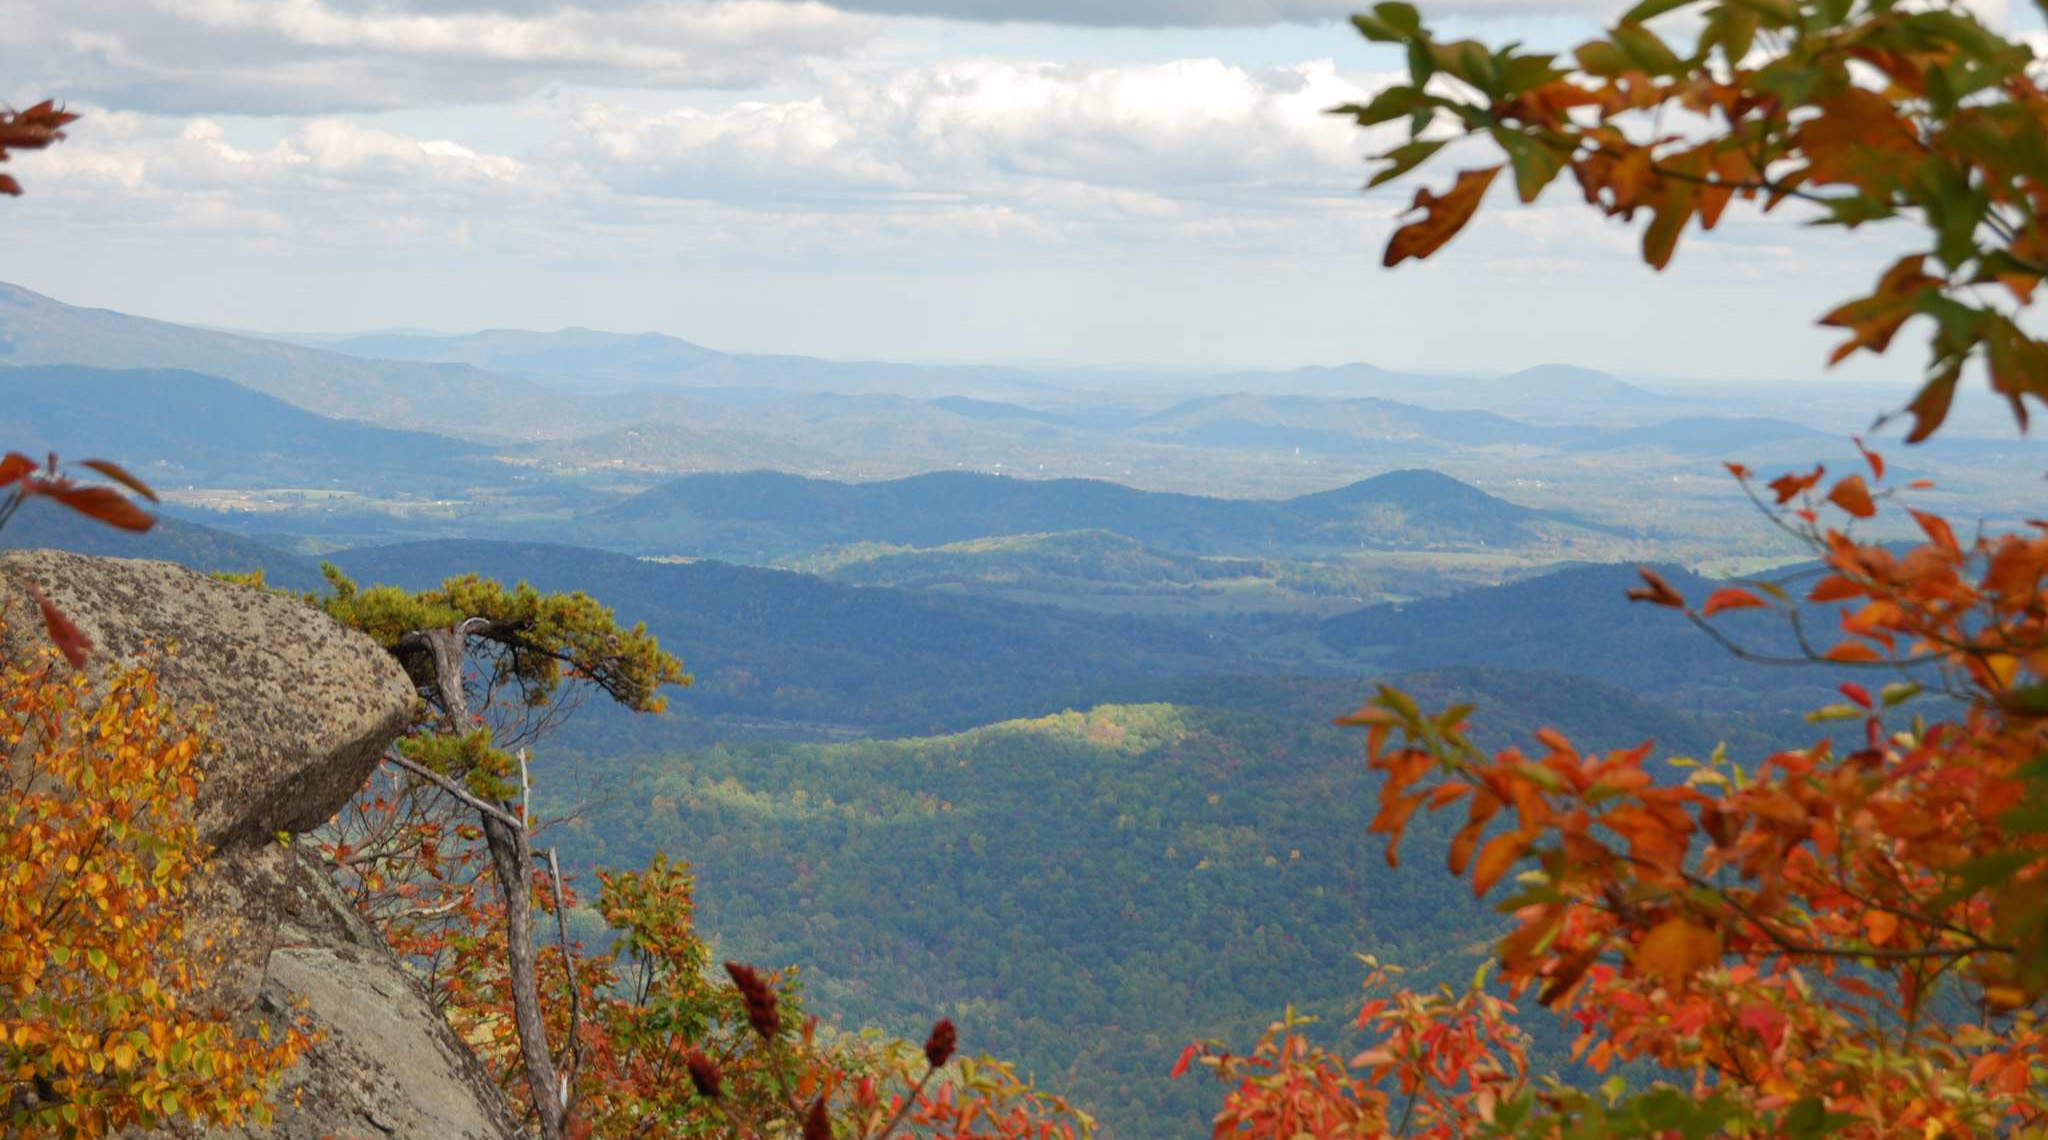
\includegraphics[width=\linewidth]{view}
%\caption{Wide Picture}
%\label{fig:view}
%\end{figure*}

%\lipsum[4] % Dummy text
%\vspace{5cm}

This section is separated into 3 steps:
\begin{enumerate}[noitemsep] % [noitemsep] removes whitespace between the items for a compact look
\item Imaging the phantom and preprocessing
\item ImpactMC simulation
\item Analysis of the results
\end{enumerate}

%\begin{description}[noitemsep]
%\item[Section 1, the phantom] Imaging the phantom and preprocessing
%\item[Section 2, simulation] ImpactMC simulation
%\item[Section 3, the results] Analysis of the results
%\end{description}

\section{Methods and theory, preprocessing}
This section covers all the processing needed to be done before the simulation.

\subsection{CT imaging principle}
Let's start with the small snap of theory about Computed Tomography (CT) imaging. The CT-imaging bases on ability of X-ray to pass through the object without significant change of the ray direction, and proportional to signal weakening while passing through material. In other words, there are two assumed postulates:
\begin{enumerate}[noitemsep] % [noitemsep] removes whitespace between the items for a compact look
\item X-ray direction doesn't change while passing through the object
\item The X-ray attenuation proportionally depends on the density of the passed material.
\end{enumerate}

Those assumptions result in situation illustrated in Fig. \ref{fig:Tomo_1}
\begin{figure}[ht]\centering
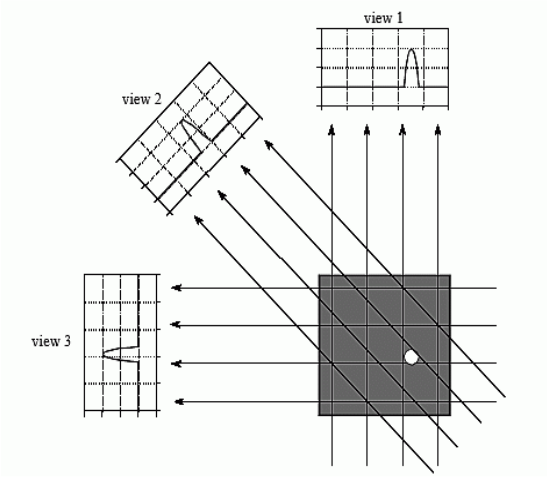
\includegraphics[width=0.9\linewidth]{Tomo_1}
%\missingfigure{Eunice phantomin kaksi 3D kuvaa vierekkäin}
\caption{The imaging principle of CT.}
\label{fig:Tomo_1}
\end{figure}
%% http://www.dspguide.com/ch25/5.htm

The next step is the inverse problem of combining the multiple directional scans into forming the image. The simple version of reconstruction called "Backprojection" is illustrated in Fig. \ref{fig:Tomo_2}.

\begin{figure}[ht]\centering
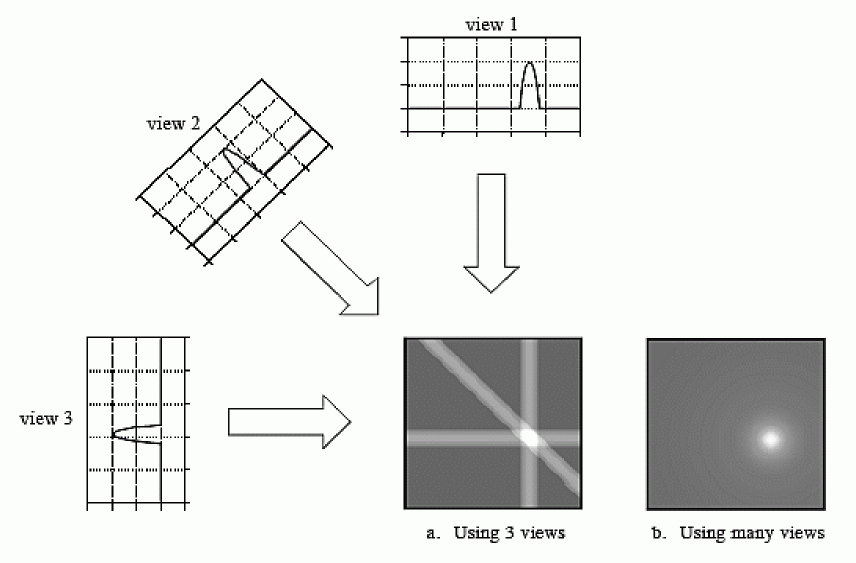
\includegraphics[width=0.9\linewidth]{Tomo_2}
%\missingfigure{Eunice phantomin kaksi 3D kuvaa vierekkäin}
\caption{The reconstruction principle of CT.}
\label{fig:Tomo_2}
\end{figure}
%% http://www.dspguide.com/ch25/5.htm

Nowadays, the reconstruction algorithms are not that simple, there are many filterings applied in order to improve the image quality. In more detail, the reconstruction algorithms are described in the course "Inverse problems" by Samuli Siltanen, Math department at the University of Helsinki.


\subsection{Eunice phantom}

\subsubsection{The structure}
The Eunice phantom is a combination of plastic disks with holes for dose measurement wires. (Fig. \ref{fig:EuniceReal}) The consistance of each disk is different and reproduces the organ densities.

\begin{figure}[ht]\centering
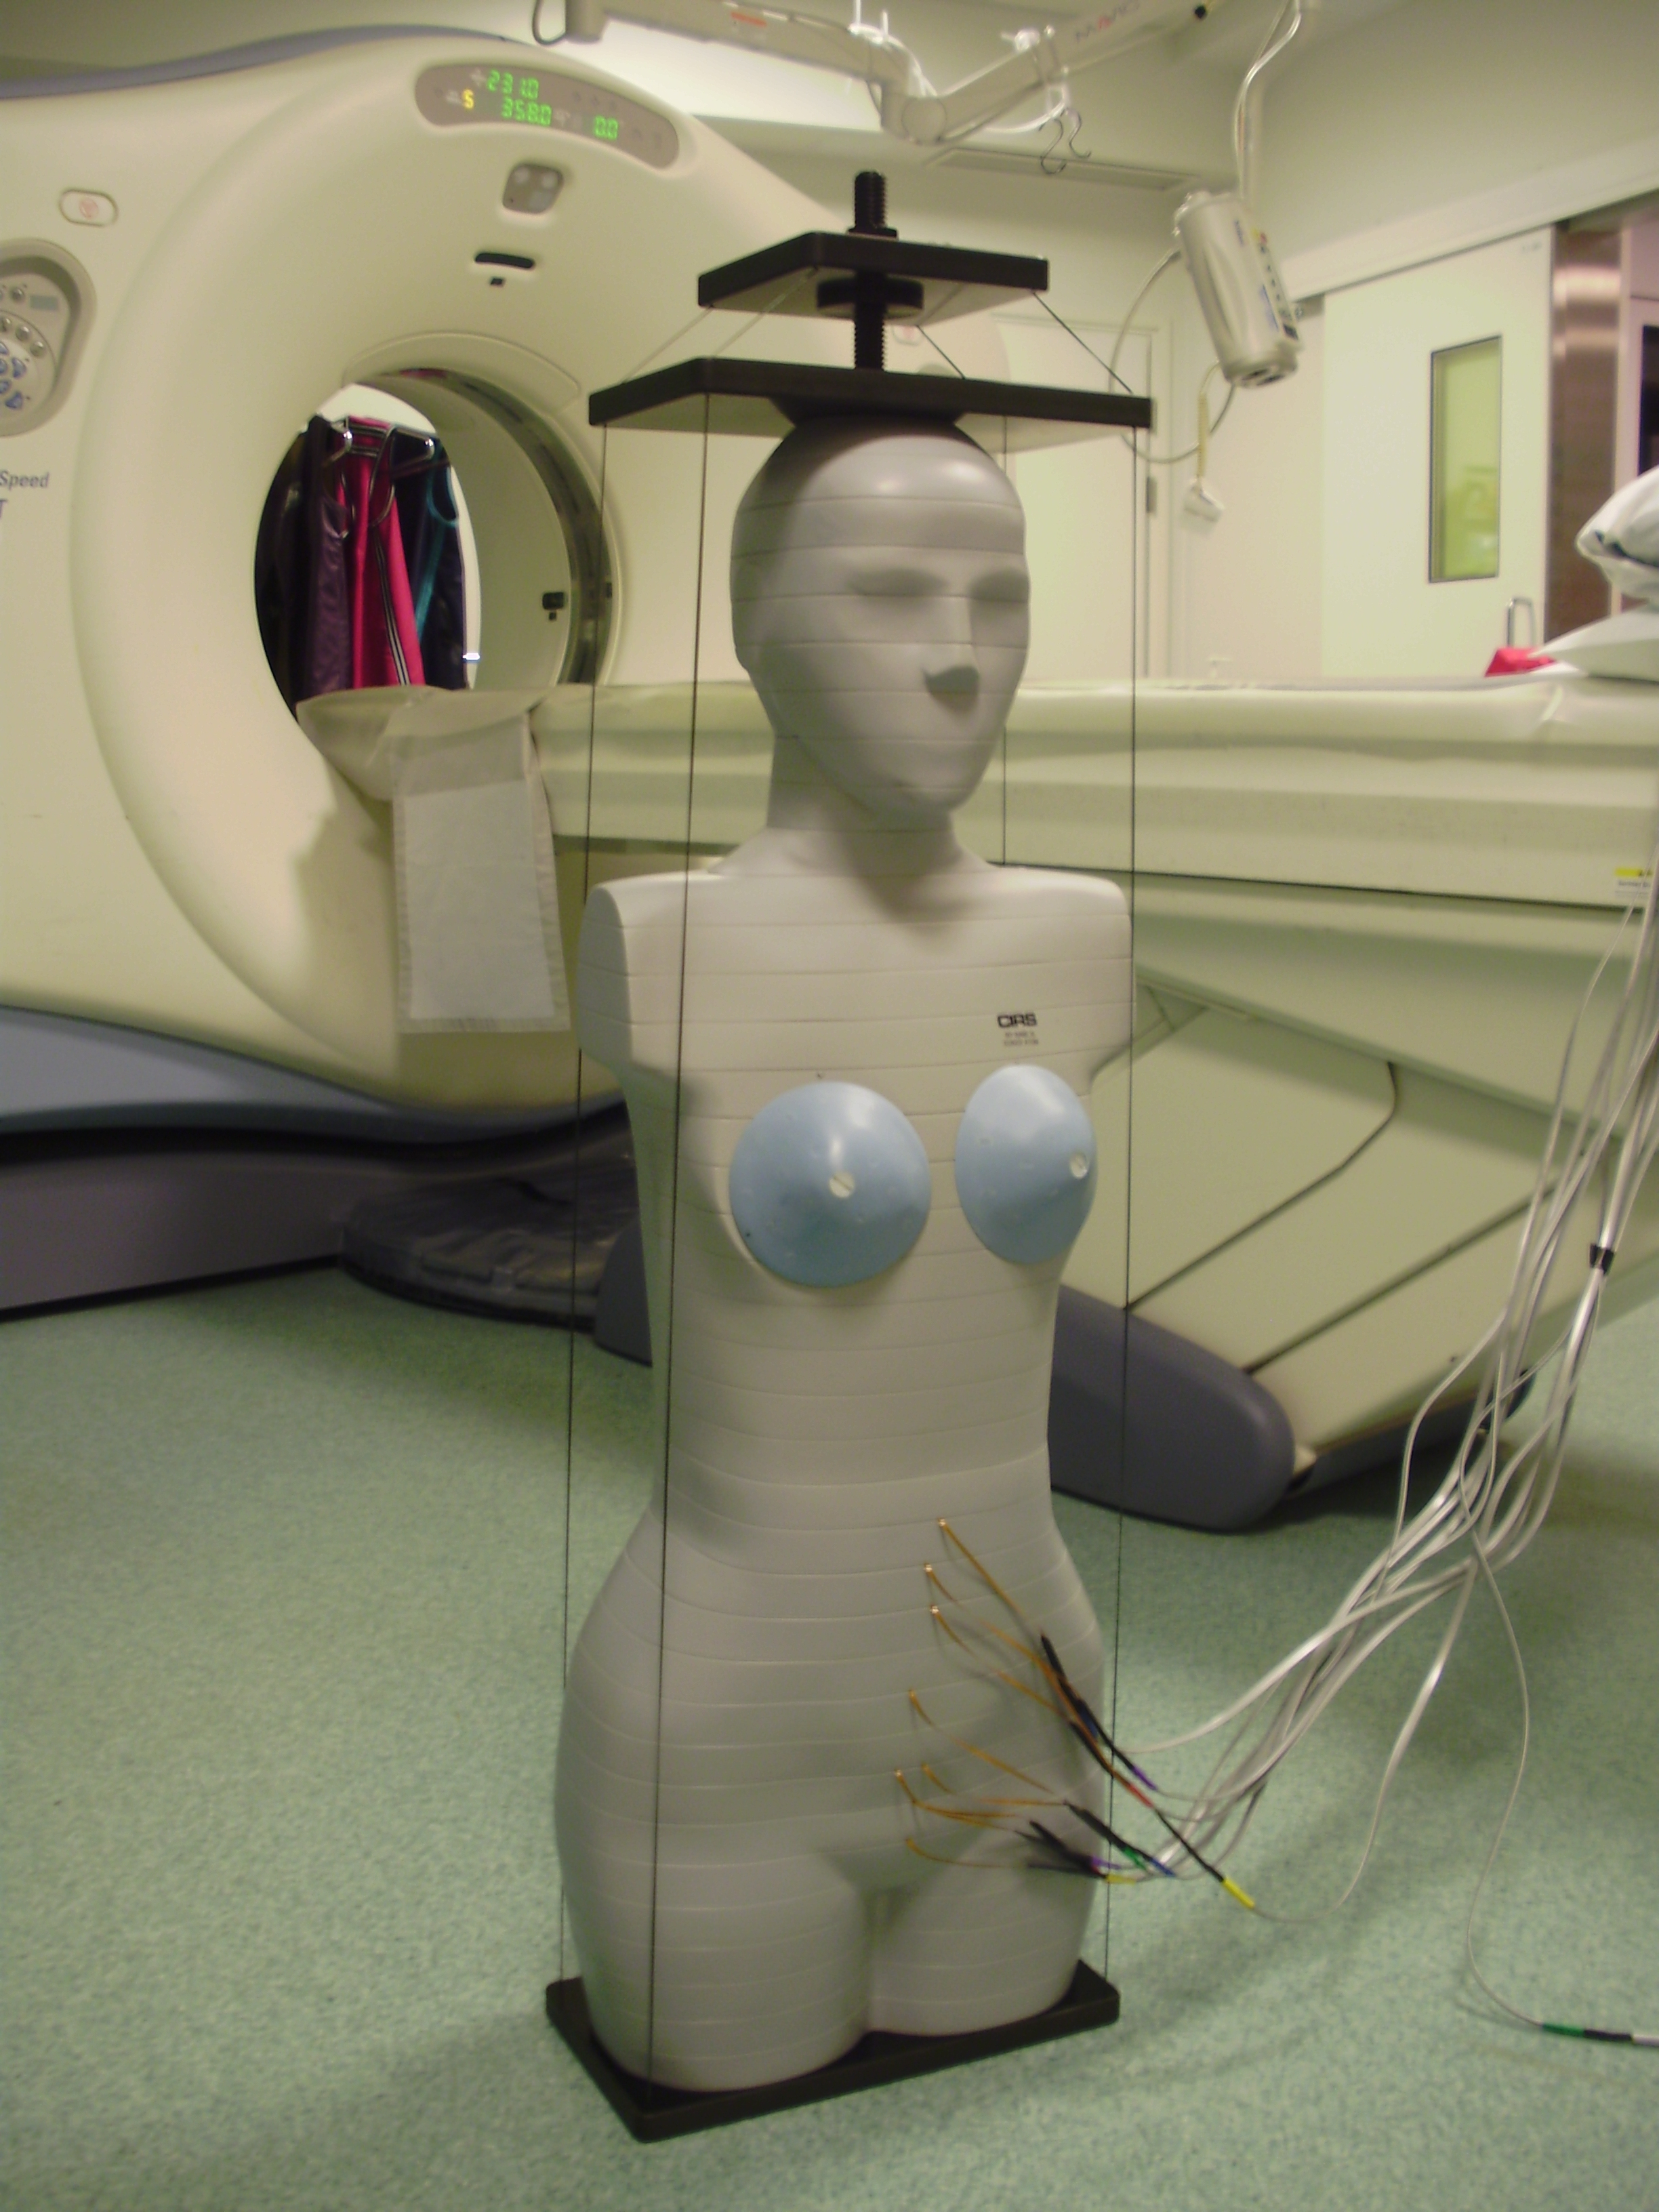
\includegraphics[width=0.9\linewidth]{EuniceReal}
%\missingfigure{Eunice phantomin kaksi 3D kuvaa vierekkäin}
\caption{A photo of the Eunice phantom.} 

\label{fig:EuniceReal}
\end{figure}
%\todo[color=orange!60]{Anna antoi luvan kuvan käyttöön, miten viittaan siihen?}


\subsubsection{In general}
The first step is to obtain the image of the object of the investigation, in other words to get a 3D image of the phantom. The best results for the studies are produced at 129kV (Annan viitteet), however at equipment available at HUS, such sequence is not an option. The closest options are 120kV and 140 kV. Thus, for the analysis the 120kV sequence has been chosen.

The obtained image is illustrated in Fig. \ref{fig:EunicePhantom}. (Thanks to Timo Paasonen for measurement.) The dimensions of the image are 512-512-377, with voxel size of 1.5625mm-1.5625mm-2.5mm.

\begin{figure}[ht]\centering
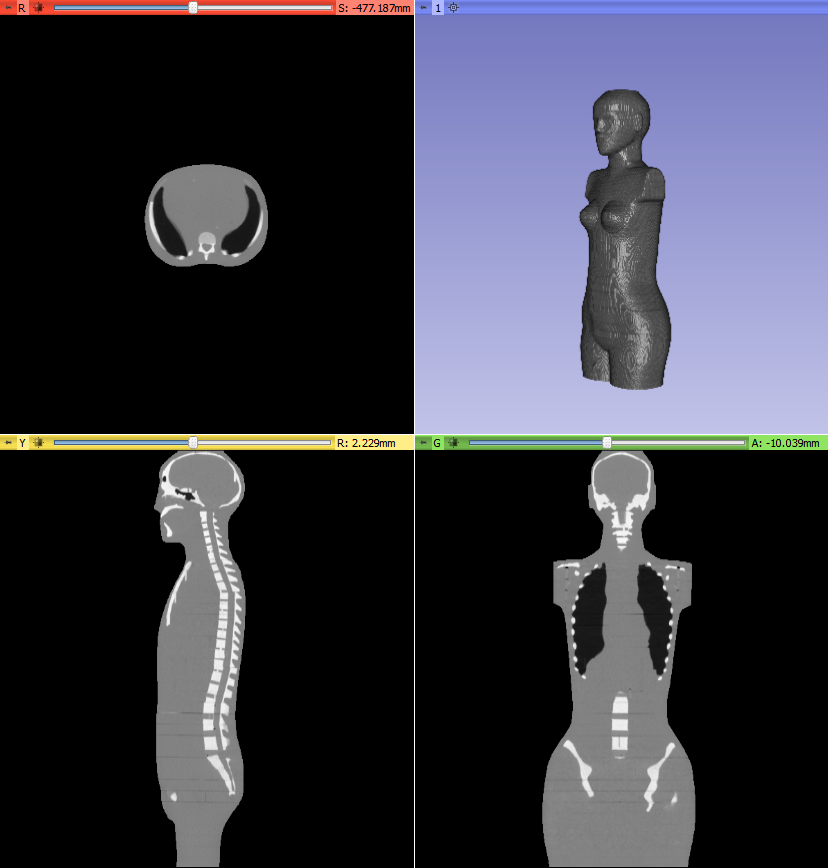
\includegraphics[width=0.9\linewidth]{Eunice}
%\missingfigure{Eunice phantomin kaksi 3D kuvaa vierekkäin. Tai nelinäkymä...}
\caption{The structure of Eunice phantom visualized as 3D image with axial (red), sagittal (yellow) and coronal (green) slices.}
\label{fig:EunicePhantom}
\end{figure}


%\begin{equation}
%\cos^3 \theta =\frac{1}{4}\cos\theta+\frac{3}{4}\cos 3\theta
%\label{eq:refname2}
%\end{equation}

%\lipsum[5] % Dummy text

%\begin{enumerate}[noitemsep] % [noitemsep] removes whitespace between the items for a compact look
%\item First item in a list
%\item Second item in a list
%\item Third item in a list
%\end{enumerate}




\subsection{CT imaging direction}

%\lipsum[6] % Dummy text
%\vspace{5cm}

The radiation dose effect is tissue dependable (VIITTEET), thus the imaging direction is chosen to be posterior-anterior. (Fig. \ref{fig:KuvausSuunta}) The benefit of such selection is minimization of the dose to baby or to a radiation sensitive organ.


\begin{figure}[ht]\centering
%\includegraphics[width=0.9\linewidth]{RGB_CellData}
\missingfigure{Mikan esitelmän kuva, jossa phantomi ja TT selästä. Muista heiluntanuolet.(kun kuvaus ei tapahdu yhdestä suunnasta vaan välistä, niin sen on hyvää näyttää.)}
\caption{The CT-imaging session.}
\label{fig:KuvausSuunta}
\end{figure}


%%\paragraph{Spectrum\\}
%%% \lipsum[7] % Dummy text
%%. \vspace{50mm} 
%%.
%%
%%\paragraph{Beam geometry\\}
%%% \lipsum[7] % Dummy text
%%.
%%\vspace{50mm}
%%.
%%
%%\paragraph{Muu} %\lipsum[8] % Dummy text
%%.
%%\vspace{50mm}
%%.
%%
%%\subsection{Object model}
%%- fantomin malli
%%%\lipsum[9] % Dummy text
%%.
%%\vspace{50mm}
%%.
%%
%%\subsection{MC simulation}
%%.
%%\vspace{50mm}
%%.




\subsection{Types of external shields}

This paper analysis the four types of external shields, based on their height. The Eunice phantom consists of 38 disks, so the types of shields are defined accordingly: A (disks 21-38), B (23-38), C (24-38), D (25-38) and K (loose D \todo[color=red!70]{vai B?}). (Fig.\ref{fig:Shields}.)

\begin{figure}[!hbt]\centering
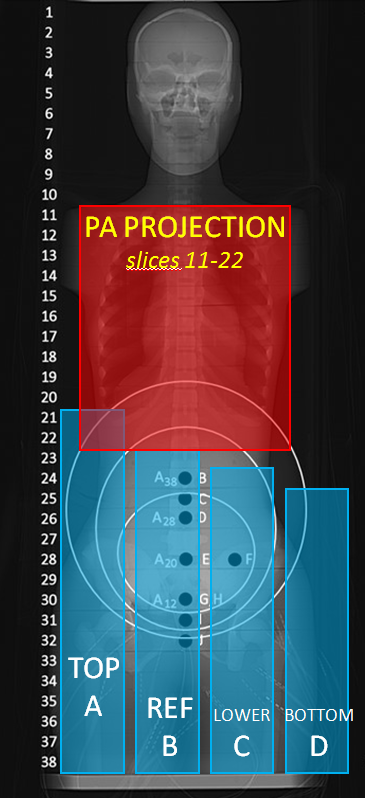
\includegraphics[width=0.9\linewidth]{Shields}
\caption{Types of shields}
\label{fig:Shields}
\end{figure}

%Reference to Figure \ref{fig:results}.


%------------------------------------------------

\section{Methods and theory, the simulation}


The general idea of the simulation is simple:
\begin{enumerate}[noitemsep]
\item Using spectrum create n-amount of particles
\item Pass them through the object
\item Record the result
\end{enumerate}

However, at a closer look, several questions like "What spectrum?", "How many particles?" and "How do they interact?" arise. This section will try to answer to those questions

\subsection{Spectrum}

The model for spectrum is obtained from XXXXXX, and it's probability density function is illustrated in Fig. \ref{fig:Spectrum}.

\begin{figure}[ht]\centering
%\includegraphics[width=\linewidth]{spectrumImage}
\missingfigure{Spektrin kuva}
\caption{The probability density function of X-ray particles for 120kV energy.}
\label{fig:Spectrum}
\end{figure}


\subsection{Number of simulation particles}

In the literature, the most common limitation for the simulation is the processing time, not the amount of particles.(VIITTEET) However, such approach is not practical, since it limits the reproducibility on another machine.

For this reason, we evaluated at a range from 10e8 to 10e11 and observed the results in Fig \ref{fig:PhotonNumber}. 

\begin{figure}[!hbt]\centering
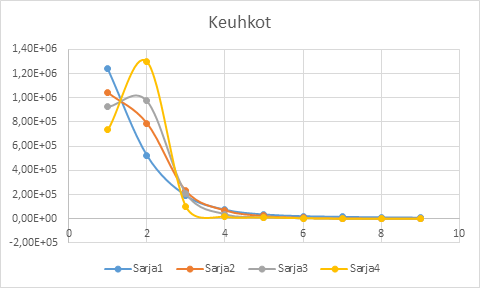
\includegraphics[width=\linewidth]{PhotonNumber}
%\missingfigure{Spektrin kuva}
\caption{Normalized dose distributions from 10e8 to 10e11 in the chest.}
\label{fig:PhotonNumber}
\end{figure}

\todo[inline]{Paivita kuva kun saadaan uudet laskut valmiiks... [Huom. 1e8,5e8, harmaa on 1e9, kultainen 1e10.] }

From this image we can clearly conclude that the structure of the curve doesn't significantly change from the 10e9, thus that amount of particles we use in following simulations.

\subsection{Physics of interaction}
\textit{\textbf{Rayleigh sironta (klassinen sironta), suora beamin, sironta (scattering)
}}.
.

\subsection{Step-by-step guide}
For some strange reason the GPU version works well only with folders located on the desktop. Thus:\\
\textbf{1. Create root folder on desktop (any name) and place all data inside. Especially phantom's dcm-images should be placed inside  \textit{Input}  folder. }\\
The situation is illustrated in image: \\
\begin{figure}[ht]\centering
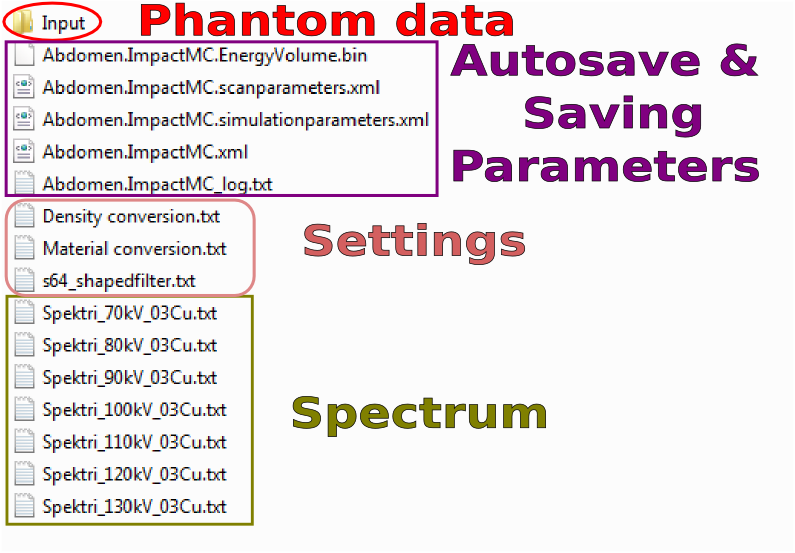
\includegraphics[width=\linewidth]{folderStructure}
\caption{The project root folder locating on the Desktop}
\label{fig:folderStructure}
\end{figure}

The content of Figure \ref{fig:folderStructure} can be classified into 4 blocks:
\begin{enumerate}
\item The folder with phantom data in dicom format (Red)
\item Saving details\\
-- This eliminates the need to manually set parameters at each launch.\\
-- And allows to resume work from the stop point.
\item Settings\\
-- Density Conversion settings (more detailed described in files of Figure \ref{fig:folderStructure}, part \textit{"Settings"})\\ 
Practically since we assume that shield is plumbum, the transformation term into plumbum is added.\\
-- Material Conversion table\\
-- shapefilter\\
\item Spectrum tables for each energy\\
-- The simulation is meant to be done on several energies

\end{enumerate}


\begin{table}[!hbt]
\caption{Material conversion settings}
\centering

   \label{tab:label}
   \begin{tabulary}{\linewidth}[hbt]{||c|c||}
  \hhline{|t:==:t|}
   \textbf{Variable} & \textbf{Parameter}\\
  %\hhline{|t:==:t|}
  \hhline{|:=|=:|}
    Air &  -900\\
%  \hline
%    \multicolumn{2}{|l|}{7 8}\\
	\hhline{||--||}
   H20 & 200\\
	\hhline{||--||}
  Bone & 3000\\
	\hhline{||--||}
  Lead & 64535\\
  \hhline{|b:==:b|}
  \end{tabulary}
\end{table}


\textbf{2. Now we can launch the GUI version of ImpactMC. }

\begin{figure}[ht]\centering
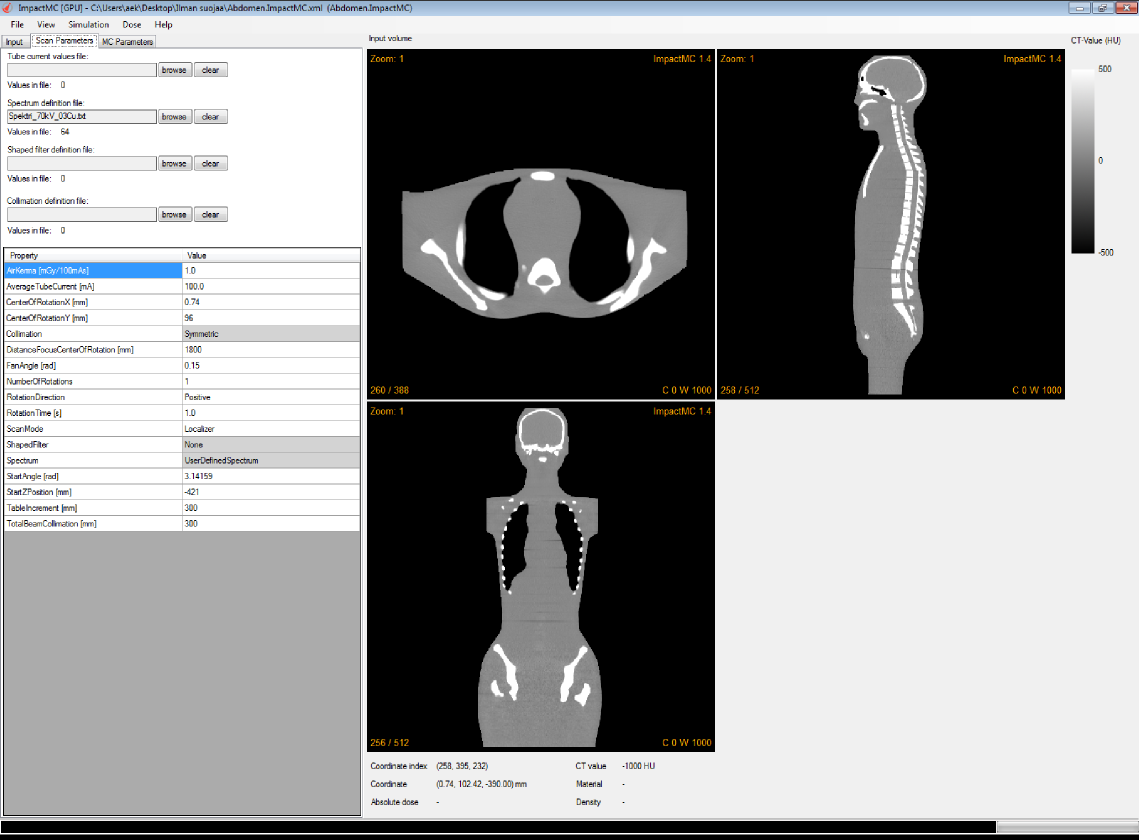
\includegraphics[width=\linewidth]{startingImage}
\caption{The starting project window}
\label{fig:startingImage}
\end{figure}
This graphical user interface consists of 2 blocks: Visualization on the right, and the tabbed parameter setting form on the left. The transfer between MRI image of phantom and dose simulation is performed through the menu options on the top.\\
 \textit{Note: This software produces report message about each completed task and tilts in case some action is taken inside it during the simulation, so waiting for the report is highly recommended.}
%\lipsum[10] % Dummy text


% http://tex.stackexchange.com/questions/79369/formatting-table-border-and-text-alignment-in-latex-table




%\begin{table}[hbt]
%\caption{Second tab of settings}
%\centering
%
%   \label{tab:label}
%   \begin{tabulary}{\linewidth}[hbt]{||c|c||}
%  \hhline{|t:==:t|}
%   \textbf{Variable} & \textbf{Parameter}\\
%  %\hhline{|t:==:t|}
%  \hhline{|:=|=:|}
%    1 &  4\\
%%  \hline
%%    \multicolumn{2}{|l|}{7 8}\\
%	\hhline{||--||}
%   9 & 12\\
%	\hhline{||--||}
%  13 & 16\\
%  \hhline{|b:==:b|}
%  \end{tabulary}
%\end{table}
%
%
%\begin{table}[hbt]
%\caption{Third tab of settings}
%\centering
%
%   \label{tab:label}
%   \begin{tabulary}{\linewidth}[hbt]{||c|c||}
%  \hhline{|t:==:t|}
%   \textbf{Variable} & \textbf{Parameter}\\
%  %\hhline{|t:==:t|}
%  \hhline{|:=|=:|}
%    1 &  4\\
%%  \hline
%%    \multicolumn{2}{|l|}{7 8}\\
%	\hhline{||--||}
%   9 & 12\\
%	\hhline{||--||}
%  13 & 16\\
%  \hhline{|b:==:b|}
%  \end{tabulary}
%\end{table}



.
\vspace{10mm}
.\\
\textbf{
\emph{To be continued, kopioi Alexey\_labra.doc tänne nätisti.
}}\\
.
\vspace{10mm}
.



%%%%%   Table temlate  %%%%%%%%%%%%%%%%%%%%%%
%%%\documentclass{article}
%%%\usepackage{xcolor}
%%%\usepackage{dcolumn}
%%%\usepackage{tabu}
%%%
%%%\newcolumntype{A}{D{.}{.}{2.3}}
%%%
%%%\begin{document}
%%%
%%%\begin{table}[htbp]
%%%  \centering
%%%  \caption{Distribution of Number of Injured Non-Motorists by Injury Severity Level}
%%%    \extrarowsep=_3pt^3pt
%%%     \begin{tabu}to\linewidth{|[2pt gray]r|c|A|c|A|c|A|[1.5pt gray]}
%%%    \tabucline[1.5pt gray]-
%%%    \bfseries Injury Severity  & \multicolumn{2}{c|}{\textbf{Pedestrian}} & \multicolumn{2}{c|}{\textbf{Bicyclist}} & \multicolumn{2}{c|[1.5pt gray]}{\textbf{All Non-Motorists}} \\
%%%    \tabucline[1.5pt gray]-
%%%    Possible injury & 1700  & 67.70\% & 502   & 59.40\% & 2202  & 65.60\% \\
%%%    Non-Incapacitating injury & 523   & 20.80\% & 259   & 30.70\% & 782   & 23.30\% \\\hline
%%%    Incapacitating injury & 250   & 10.00\% & 84    & 9.90\% & 334   & 9.90\% \\\hline
%%%    Fatal injury & 39    & 1.50\% & 0     & 0.00\% & 39    & 1.20\% \\
%%%    \tabucline[1.5pt gray]-
%%%    \bfseries Total & \bfseries 2512 & \multicolumn{1}{c|}{\bfseries 100.00\%} & \bfseries 845 & \multicolumn{1}{c|}{\bfseries 100.00\%} & \bfseries 3357 & \multicolumn{1}{c|[1.5pt gray]}{\bfseries 100.00\%} \\
%%%    \tabucline[1.5pt gray]-
%%%    \end{tabu}%
%%% \label{tab:dvar}%
%%%\end{table}%
%%%
%%%\end{document}



%.
%\vspace{30mm}
%.
%


%------------------------------------------------

\section{Methods and theory, the analysis}
In this section we briefly describe the methodology used in result analysis. The main guidelines of wanted results are the doses in organs and dose distribution maps.

\subsection{Organ doses}
\label{subsec:OrganDoses}
The first step in calculating organ doses is locating those organs in measured CT image. In this paper it is done manually following the guidelines presented in the Eunice phantom documentation (VIITE).

This operation is called volumetric analysis. The volumetric analysis means that each object is segmented from the context, and investigated separately. Such approach provides more detail information about the organ, and allows to investigate maximal accursed doses in a regions.

\subsection{Voxel-based analysis}

%This doses can be processed in a two way:
%\begin{enumerate}
%\item Volumetrically, as a dose distribution over an organ. The aim is to get some precise values.
%\item Histogrammically, which means volumetrically, but also as a function of the imaging energy. For a better precision, the dose distribution is invistigated per voxel. This method provides a comparison of effects from different imaging energies.
%\end{enumerate}


%The histogrammical analysis means that every voxel is a measurement point. Basing on the intensities these points can be classified into bins. The produced results are the mean values of the volumes.

This approach is sometimes called histogrammic analysis. The idea is to investigate the image on a voxel size, and create a histograms based on a suitable binning. There are several goals of such analysis:

\begin{enumerate}[noitemsep]
\item Analyze the dose distribution.
\begin{enumerate}[noitemsep]
\item Easy check if the simulation obeys common sense rules.
\item Verifying how the organ dose is formed. = Verifying that the dose is semi-equally distributed over the organ, and not formed as a pack of high and low dose values.
\end{enumerate}
\item Investigate the dose distribution behavior over the different imaging energies.
\end{enumerate}


%
%Periaatteet:\\
%- histogram\\
%- 3D image
%.
%\vspace{50mm}
%.



\subsection{Change of the 3D dosemap according to shield}
Another possibility is to analyze the effect of external shields to the dose distribution. This analysis is similar to analysis methods presented in \ref{subsec:OrganDoses}, except that in this case we are interested in the difference between shielded simulations in the same organ.




\section{Results}
The aims of this paper are to illustrate the process, to make some conclusion about external shields effect on dose and to visualize the predicted effect of the increase in the imaging energy on a dose. Current section describes the last two.
%\lipsum[10] % Dummy text

%.
%\vspace{30mm}
%.
%

\subsection{Relative doses, no shields}

The obtained simulation dose image is illustrated in Figure \ref{fig:NoShieldImage} .

\begin{figure}[!hbt]\centering
%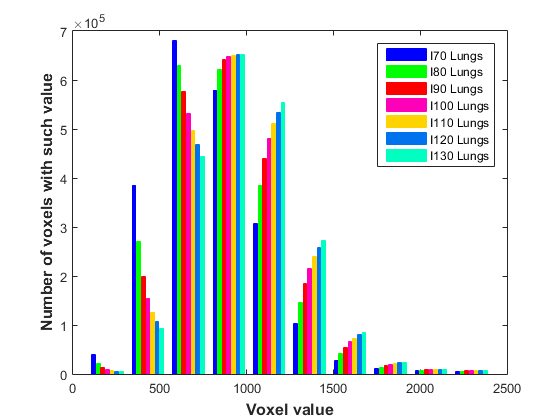
\includegraphics[width=\linewidth]{NoShieldLungs}
\missingfigure{Hieno värikäs kuva annoksesta eri puolilta, esim 2 3D}
\caption{The simulated dose distribution over the phantom.}
\label{fig:NoShieldImage}
\end{figure}


Figure \ref{fig:NoShieldLungs} demonstrates the voxel intensity (the absorbed dose) variation over the energy in lungs.

\begin{figure}[!hbt]\centering
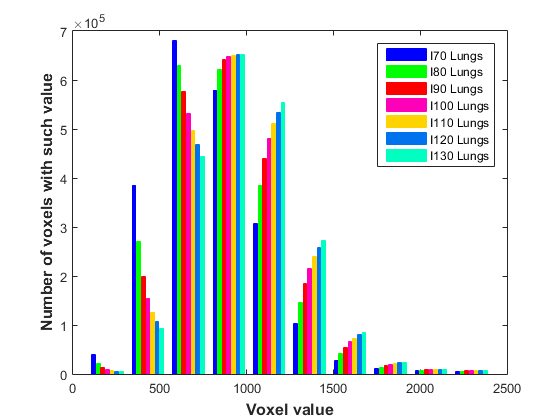
\includegraphics[width=\linewidth]{NoShieldLungs}
%\missingfigure{No shield image, histogram of lungs}
\caption{The histogrammical distribution of the dose in lungs depending on imaging energy.}
\label{fig:NoShieldLungs}
\end{figure}

As it can be noticed the increase of imaging energy results in higher dose. This conclusion makes sense.

In addition we can observe similar analysis of other organs, t.ex. liver (Figure \ref{fig:NoShieldLiver}), kidney (Figure \ref{fig:NoShieldKidneys}), breasts (Figure \ref{fig:NoShieldBreasts}).

\begin{figure}[!hbt]\centering
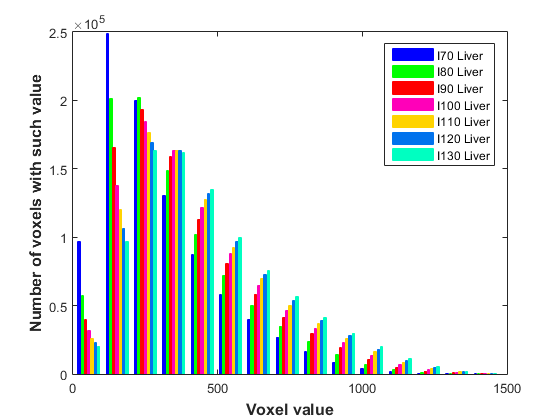
\includegraphics[width=\linewidth]{NoShieldLiver}
%\missingfigure{No shield image, histogram of liver}
\caption{The histogrammical distribution of the dose in liver depending on imaging energy.}
\label{fig:NoShieldLiver}
\end{figure}

\begin{figure}[!hbt]\centering
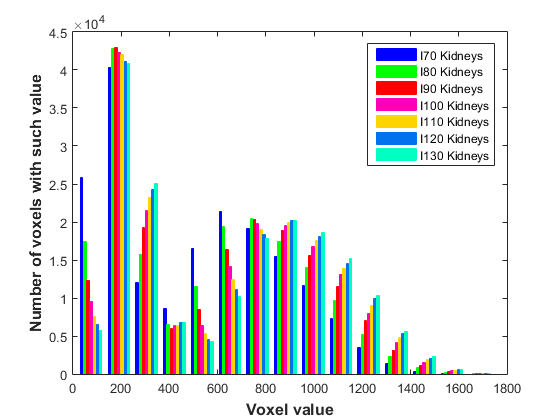
\includegraphics[width=\linewidth]{NoShieldKidneys}
%\missingfigure{No shield image, histogram of kidney}
\caption{The histogrammical distribution of the dose in kidney depending on imaging energy.}
\label{fig:NoShieldKidneys}
\end{figure}

\begin{figure}[!htb]\centering
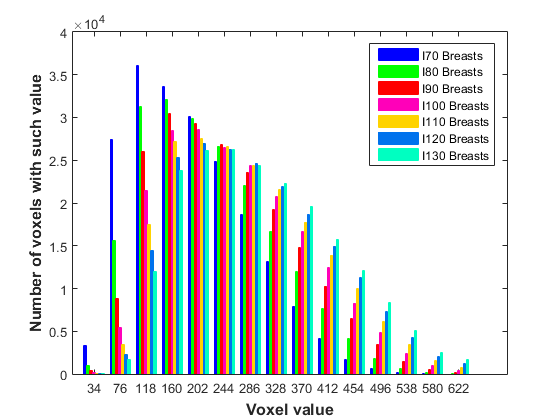
\includegraphics[width=\linewidth]{NoShieldBreasts}
%\missingfigure{No shield image, histogram of breasts}
\caption{The histogrammical distribution of the dose in breasts depending on imaging energy.}
\label{fig:NoShieldBreasts}
\end{figure}

As it can be noticed all of those organs have similar shapes of histograms, but with smaller values, since due to geometry of measurement/simulation they are further from the beam.



\subsection{Relative doses, effect of shields}

And now let's evaluate the effect of the shields on the dose.

At first let's observe the similar situation with the shields. In this particular case we use B-styled shield which provides us the following image. (Figure \ref{fig:BShieldIntensityLungs})

\begin{figure}[!htb]\centering
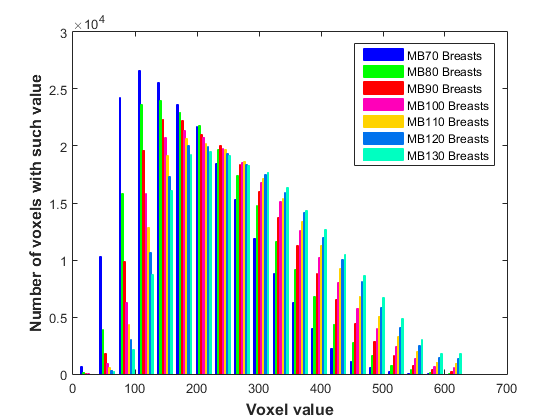
\includegraphics[width=\linewidth]{MBShieldBreasts}
%\missingfigure{No shield image, histogram of breasts}
\caption{B shield over intensity, lungs.}
\label{fig:MBShieldBreasts}
\end{figure}

We can notice that the pattern of the non-shielded version and shielded differs. The pattern of non-shielded is gaussian, meanwhile the pattern of the shielded one is significantly lowered for low intensities while remaining similar at top intensities. The top intensities are caused by the beam, which is not interacting with the shields, but the secondary radiation is filtered out by the shield.

\textbf{\textit{Voiko olettaa että ilmassa beamin leveäminen on likimain nolla? Jos voi, niin mallissa on ongelma.}}

The next subject of invetigation, is the effect of the shield type on the dose. 
Since the imaging commonly [VIITE] occurs at 120 keV \textbf{\textit{[?????], [VIITE]}}, we investigate all shield types presented in Figure \ref{fig:Shields} at that energy. The Figures \ref{fig:LungsAllShields} -- \ref{fig:LiverAllShields} illustrate the results. 

\begin{figure}[!htb]\centering
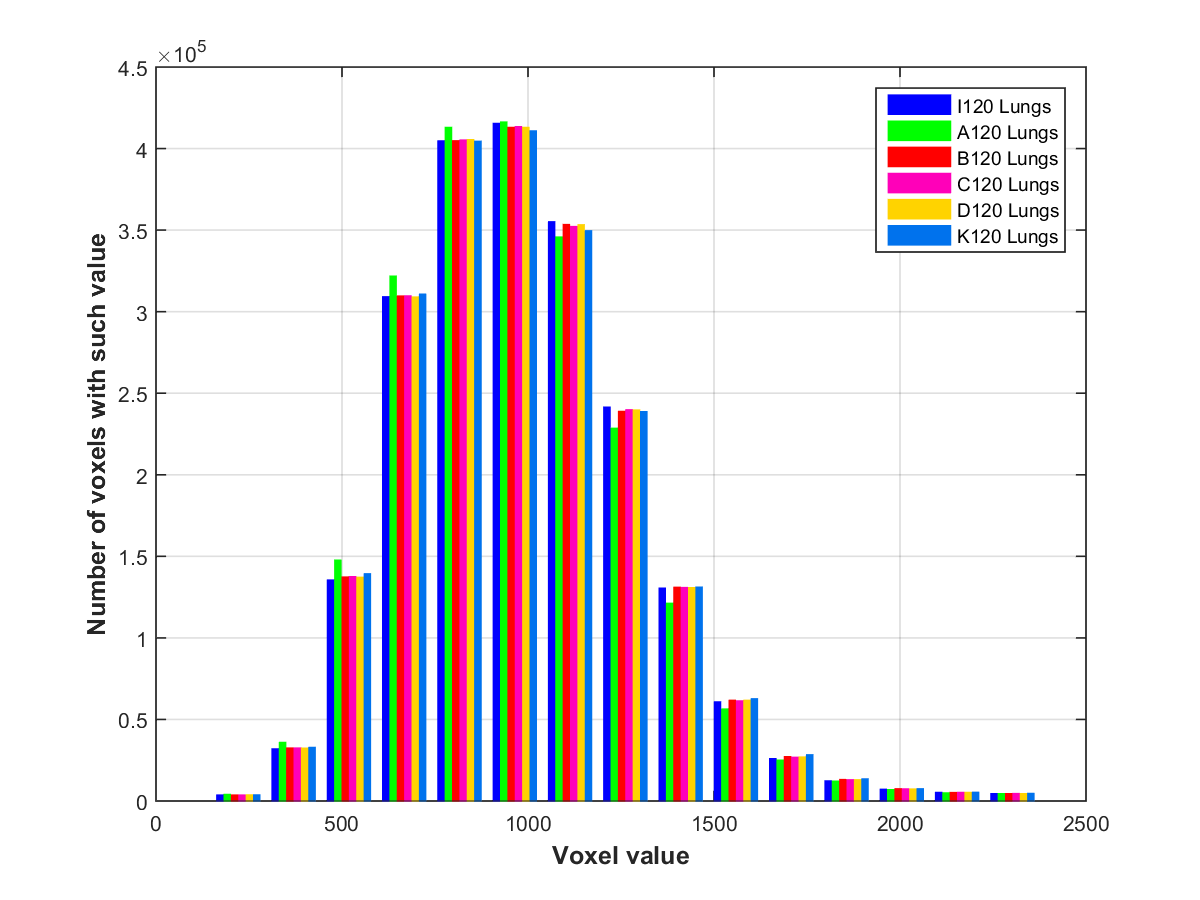
\includegraphics[width=\linewidth]{LungsAllShields}
%\missingfigure{AllShields120}
\caption{B shield over intensity, lungs.}
\label{fig:LungsAllShields}
\end{figure}

\textbf{\textit{Breasts}}

\begin{figure}[!htb]\centering
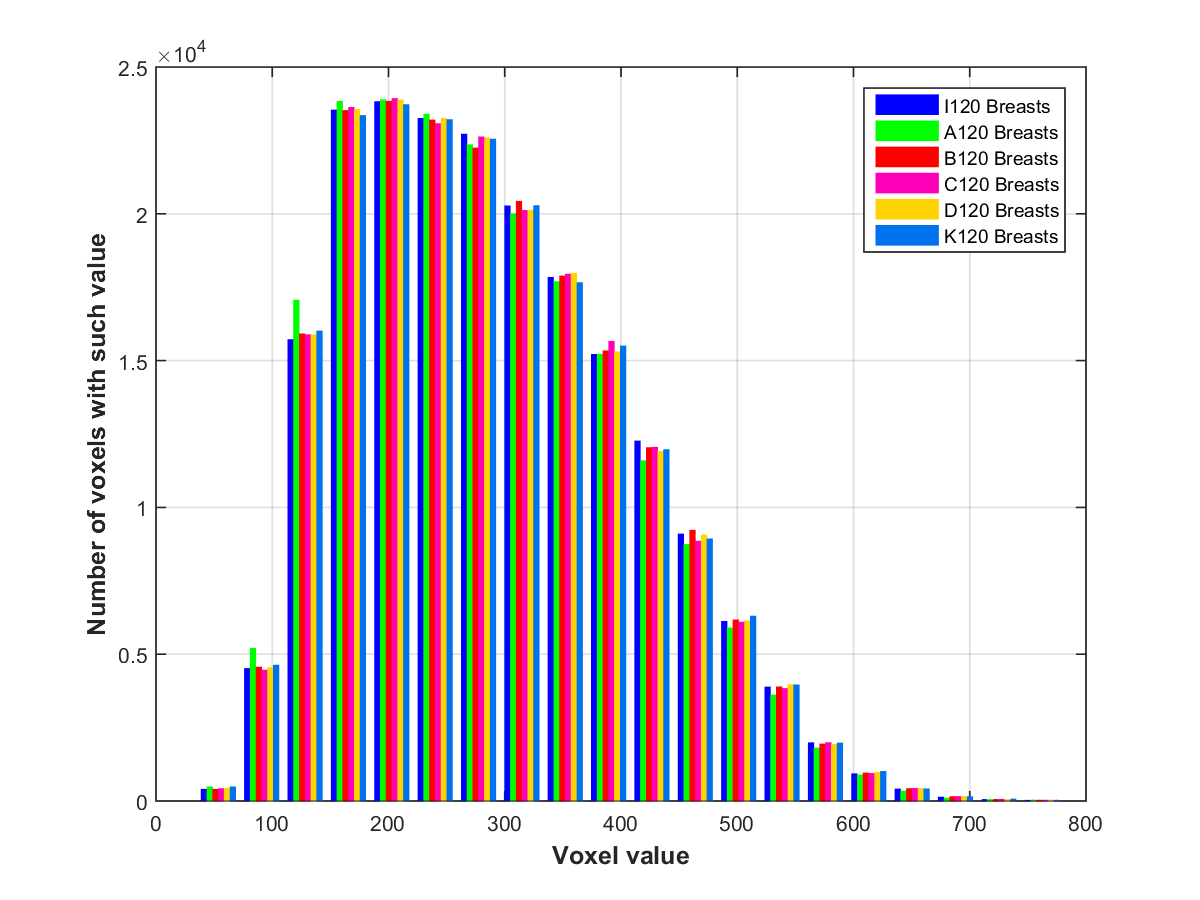
\includegraphics[width=\linewidth]{BreastsAllShields}
%\missingfigure{AllShields120}
\caption{B shield over intensity, breasts.}
\label{fig:BreastsAllShields}
\end{figure}


\textbf{\textit{Kidneys}}

\begin{figure}[!htb]\centering
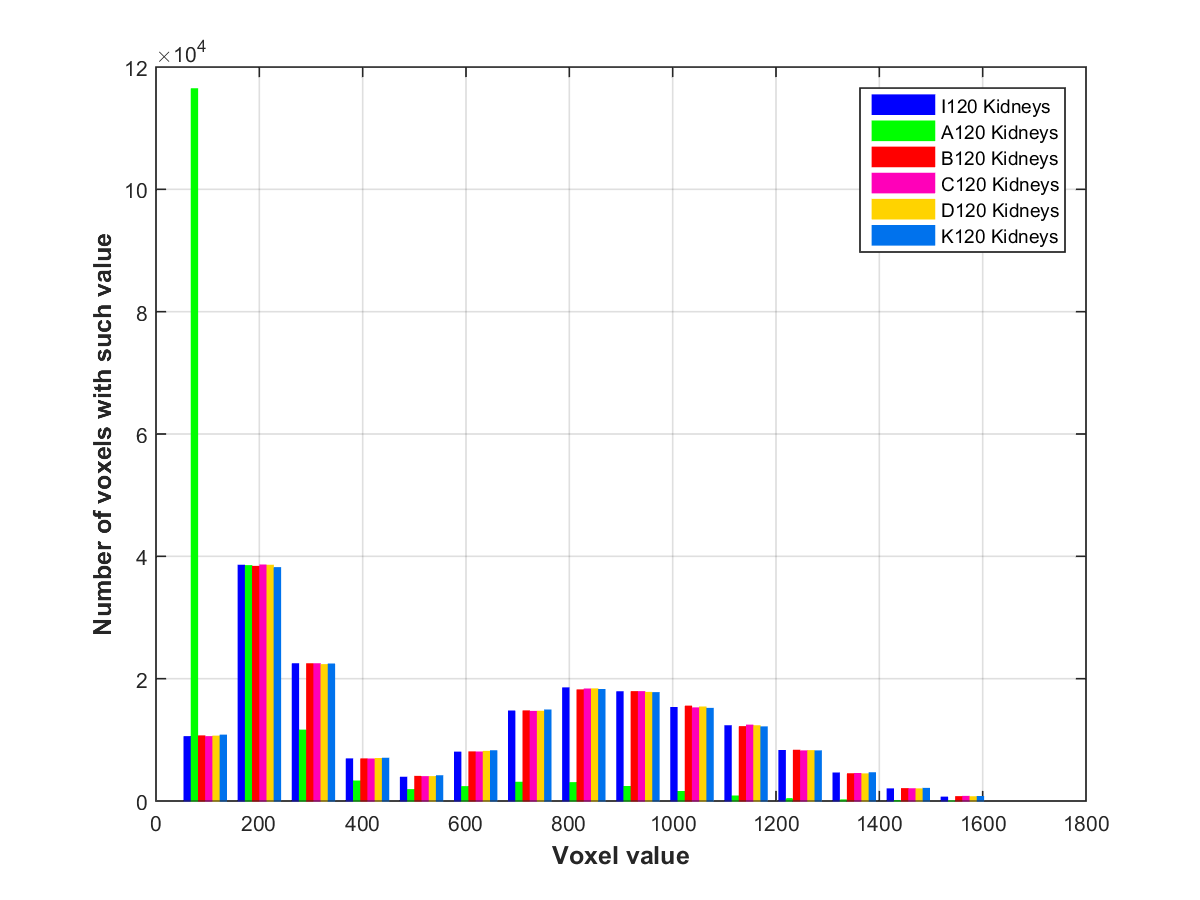
\includegraphics[width=\linewidth]{KidneysAllShields}
%\missingfigure{AllShields120}
\caption{B shield over intensity, kidneys.}
\label{fig:KidneysAllShields}
\end{figure}


\textbf{\textit{Liver}}

\begin{figure}[!htb]\centering
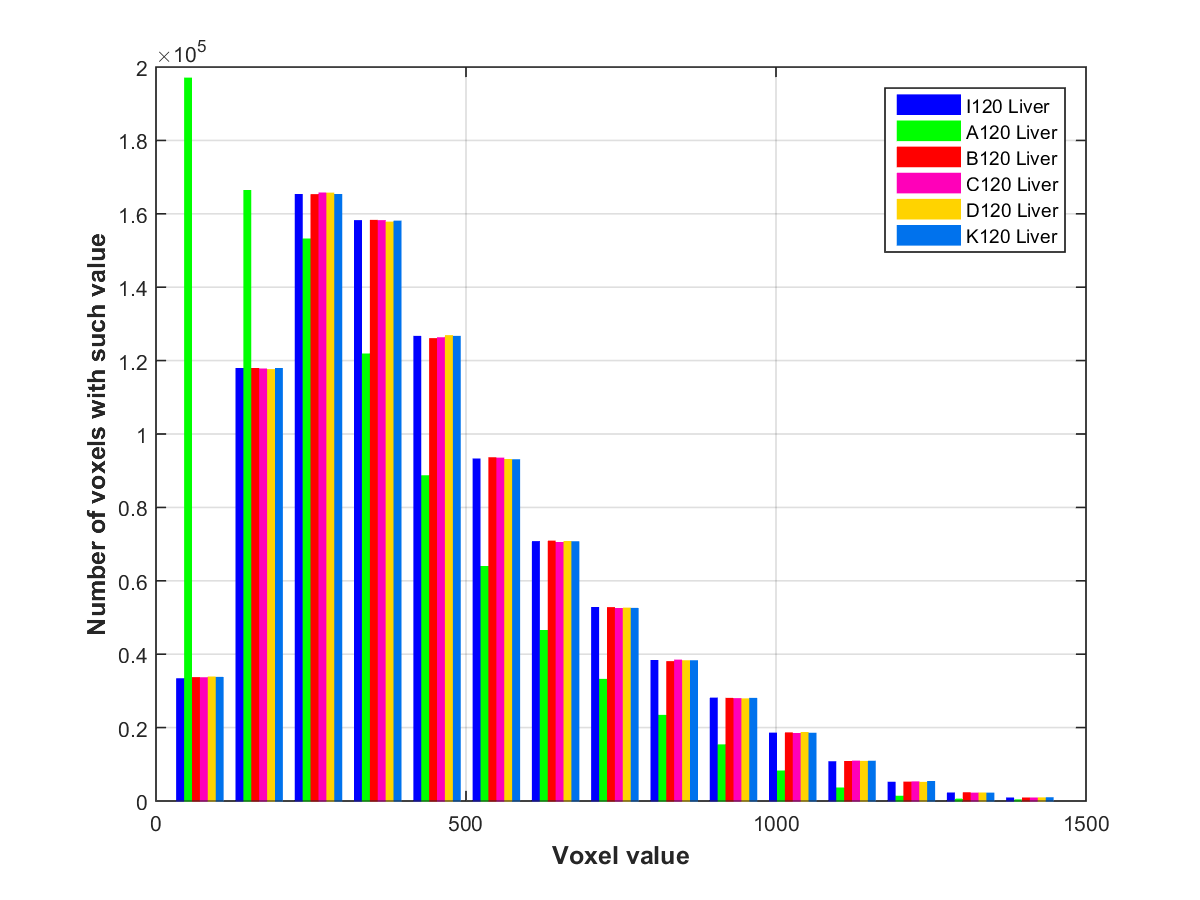
\includegraphics[width=\linewidth]{LiverAllShields}
%\missingfigure{AllShields120}
\caption{B shield over intensity, Liver.}
\label{fig:LiverAllShields}
\end{figure}


From the results we can notice that shields of type B -- D have similar effect as the lack of shields at all. The type A shield lowers the dose for kidneys, but remaining same for the rest observed organs. In next section we will analyze the dosimetrical effect of this difference.

\begin{table*}[!hbt]
	\caption{Relative dose table}
	\centering
	
	\label{tab:DoseCalculationCoefficient}
	\begin{tabulary}{\linewidth}[hbt]{||c|c|c|c|c|c|c||}
		\hhline{|t:=======:t|}
		\textbf{kV} & \textbf{A} & \textbf{B} & \textbf{C} & \textbf{D} & \textbf{No shield} & \textbf{Loose D}\\
		%\hhline{|t:==:t|}
		\hhline{|:=|=|=|=|=|=|=:|}
		70 &  &  &  &  &  &  \\
		\hhline{||-------||}
		80 &  &  &  &  &  &  \\
		\hhline{||-------||}
		90 &  &  &  &  &  &  \\
		\hhline{||-------||}
		100 &  &  &  &  &  &  \\
		\hhline{||-------||}
		110 &  &  &  &  &  &  \\
		\hhline{||-------||}
		120 &  &  &  &  &  &  \\
		\hhline{||-------||}
		130 &  &  &  &  &  &  \\
		
		
		%  \hline
		%    \multicolumn{2}{|l|}{7 8}\\
		\hhline{|b:=======:b|}
	\end{tabulary}
\end{table*}


\subsection{Absolute doses}

\subsubsection{Linkage of relative dose to absolute}

\textbf{\textit{Perustele jotenkin että pisteen valitaan teoreettisessa pisteessä sädenipun osumisesta, että häviö matkalla on pieni, häiriöiden takia maalataan pieni alue valitun pisteen paikoissa, ja se alue saa annokseksi kuvausenergian, jolloin koko matriisi vain jaetaan skaalausarvolla, niin saadaan annokset}}
\todo[color=red!70]{Mika, mihin kannattaa viitata?}

In order to obtain a prediction about the dose, we approximate the dose on the skin at perpendicular between beam and back to be 0.2 mG. (Figure \ref{fig:DoseIntensityDef}) 

\begin{figure}[!htb]\centering
	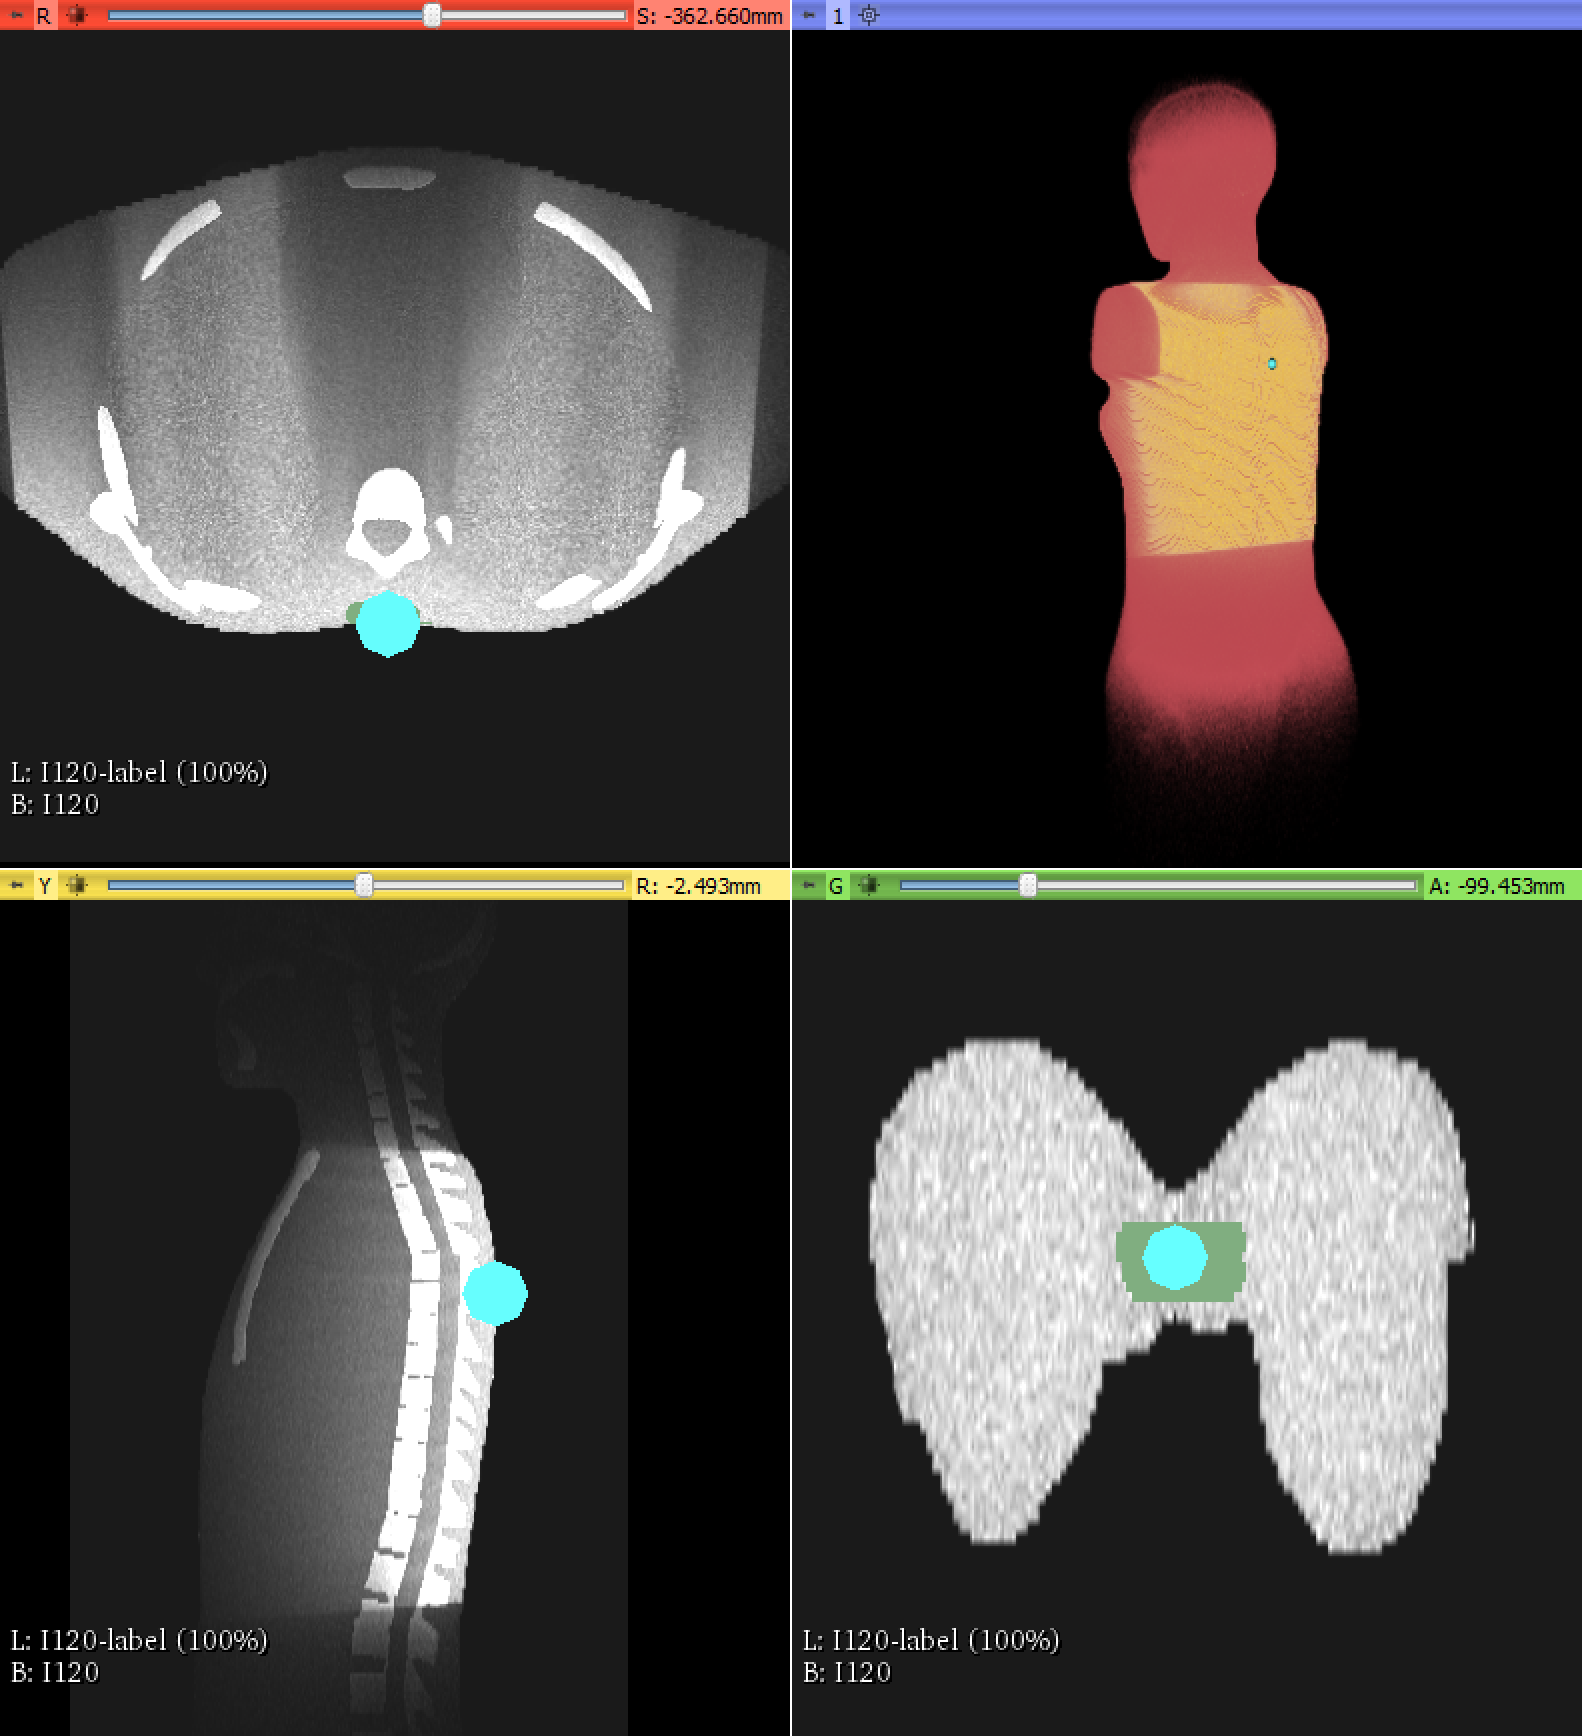
\includegraphics[width=\linewidth]{DoseIntensityDef}
	%\missingfigure{AllShields120}
	\caption{The dose definition principle from 120 kV sequence without shields. The teal dot illustrates the theoretical point of definition. However, due to noise, it is better to define an area, from which choose the intensity value.}
	\label{fig:DoseIntensityDef}
\end{figure}

The blue dot in following image illustrates the dose reference point. However to minimize the effect of the background noise, we define the area (green) and calculate the statistics over it.

\begin{table}[!hbt]
	\caption{Dose dependency on intensity definition statistics}
	\centering
	
	\label{tab:DoseCalculationCoefficient}
	\begin{tabulary}{\linewidth}[hbt]{||c|c||}
		\hhline{|t:==:t|}
		\textbf{Variable} & \textbf{Parameter}\\
		%\hhline{|t:==:t|}
		\hhline{|:=|=:|}
		Max &  2153\\
		%  \hline
		%    \multicolumn{2}{|l|}{7 8}\\
		\hhline{||--||}
		StdDev & 202.593\\
		\hhline{|b:==:b|}
	\end{tabulary}
\end{table}

From the Table \ref{tab:DoseCalculationCoefficient} we can approximate the intensity value to be

\begin{equation}
Intensity= Max - (StdDev)/2 = 2051.704
\end{equation}

This provides us Equation \ref{eq:IntensityGreyConversion}:


\begin{equation}
\begin{split}
2051.704\ intensity\ =\ 0.2\ mGy\\
\Leftrightarrow 1\ intensity\ = 9.747997... * 10^{-5}\ mGy\\
\approx 9.748 * 10^{-9} Gy = 9.748\ nGy
\end{split}
\label{eq:IntensityGreyConversion}
\end{equation}

\subsubsection{Effects on histograms in conversion between the relative and absolute doses}

The change of relative dose to absolute has no effect on histogrammical images. For example, in chest, the histogrammical approach produces Fig.\ref{fig:ChestEnergyDose}.


\begin{figure}[ht]\centering
%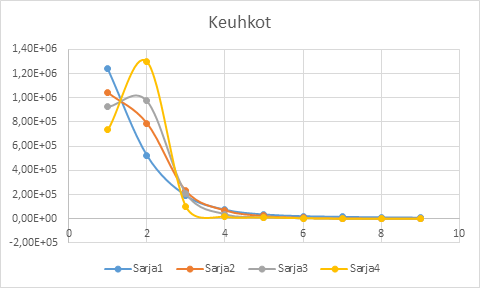
\includegraphics[width=\linewidth]{PhotonNumber}
\missingfigure{Dose distribution histogram in chest depending on energy.}
\caption{Dose distribution histogram in chest depending on energy. }
\label{fig:ChestEnergyDose}
\end{figure}
This figure is clearly same, except scaled y-axis, as the relative dose one.



%\begin{description}
%\item[Word] Definition
%\item[Concept] Explanation
%\item[Idea] Text
%\end{description}

%\lipsum[13] % Dummy text

%\begin{itemize}[noitemsep] % [noitemsep] removes whitespace between the items for a compact look
%\item First item in a list
%\item Second item in a list
%\item Third item in a list
%\end{itemize}


\subsubsection{Absolute Dose}
\textit{\textbf{Taulukko absoluuttisista annoksista}}
\begin{table*}[!hbt]
	\caption{Absolute dose table}
	\centering
	
	\label{tab:DoseCalculationCoefficient}
	\begin{tabulary}{\linewidth}[hbt]{||c|c|c|c|c|c|c||}
		\hhline{|t:=======:t|}
		\textbf{kV} & \textbf{A} & \textbf{B} & \textbf{C} & \textbf{D} & \textbf{No shield} & \textbf{Loose D}\\
		%\hhline{|t:==:t|}
		\hhline{|:=|=|=|=|=|=|=:|}
		70 &  &  &  &  &  &  \\
		\hhline{||-------||}
		80 &  &  &  &  &  &  \\
		\hhline{||-------||}
		90 &  &  &  &  &  &  \\
		\hhline{||-------||}
		100 &  &  &  &  &  &  \\
		\hhline{||-------||}
		110 &  &  &  &  &  &  \\
		\hhline{||-------||}
		120 &  &  &  &  &  &  \\
		\hhline{||-------||}
		130 &  &  &  &  &  &  \\
		
		
		%  \hline
		%    \multicolumn{2}{|l|}{7 8}\\
		\hhline{|b:=======:b|}
	\end{tabulary}
\end{table*}



\section{Discussion}
This paper presented a detailic information about the laboratory work of using simulation in computer tomography prototyping. All measurements and simulations were successful. The achieved results are in \textbf{\textit{yhteensopivat}} with the technical description of simulation software and theory predictions. In addition, the effects of the shields were analysed, \textbf{\textit{and the results suggest that ****}}. However, due to lack of statiscal significance such theory is only providing a guideline to be investigated.

\section{Future improvements}
Previous sections described the process of this laboratory work and the expected results. Thus, in this section the possible improvements will be \textit{opened}.

\subsection{Free Atlas segmentation}
In the current version the organs were manually defined based on [VIITE, Eunice ohje]. Such approach is not precise and not repeatable, thus the usage of digital phantom is recommended. There are several over the internet, but for the start taking a look at \textit{\textbf{***,***,***,***}} might be worth it.


\subsection{Variance of the model}
Each measurement of this laboratory work is done less than five times, thus we are not taking into account the variation of the ImpactMC model. For the illustration of the process/pipeline the performed analysis is enough, but for making the scientifically meaningful analysis the simulation dataset amount should be at least doubled.


%\begin{figure}[ht]\centering
%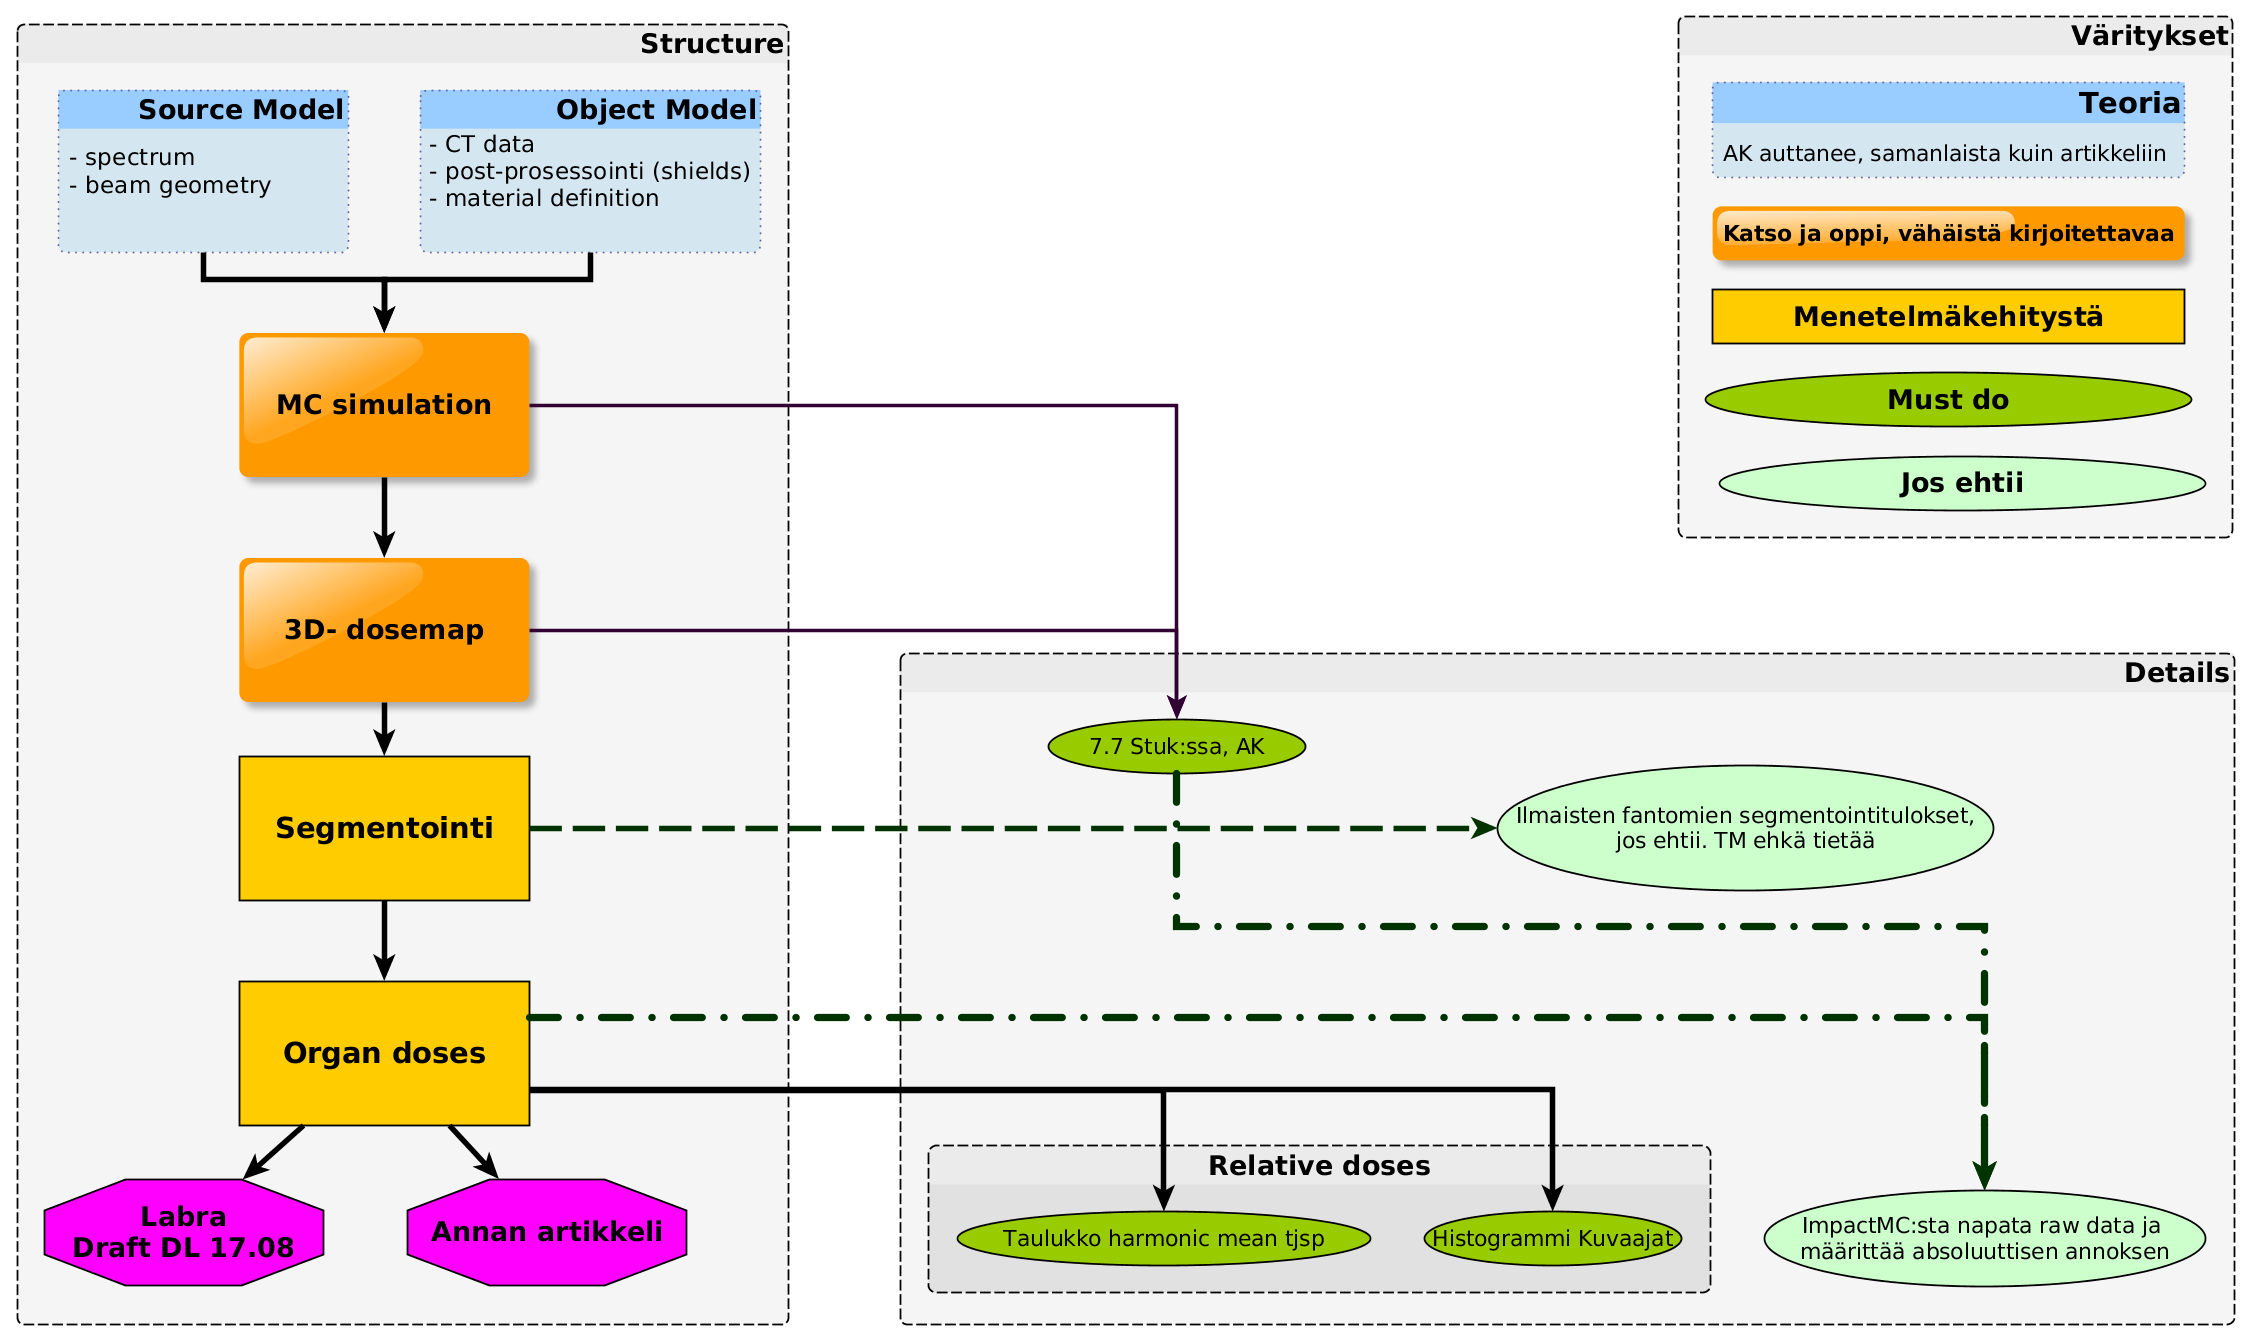
\includegraphics[width=\linewidth]{TT_SyvLabraSofiev_Plan}
%\caption{In-text Picture}
%\label{fig:TT_SyvLabraSofiev_Plan}
%\end{figure}

%\lipsum[14] % Dummy text

\subsection{Overall}
Overall, this laboratory work achieved the expectations. The ImpactMC produced truthworthful results of the dose distributions, verification and \textit{\textbf{***** jatka tänne jotain yleistä....*****}}

%\lipsum[15-23] % Dummy text

%------------------------------------------------
\phantomsection
\section*{Acknowledgments} % The \section*{} command stops section numbering

\addcontentsline{toc}{section}{Acknowledgments} % Adds this section to the table of contents

%So long and thanks for all the fish \cite{Figueredo:2009dg}.

\section*{Attachments}
\subsection*{Structure of this paper}
Fig.\ref{fig:TT_SyvLabraSofiev_Plan}.
\begin{figure*}[ht]\centering
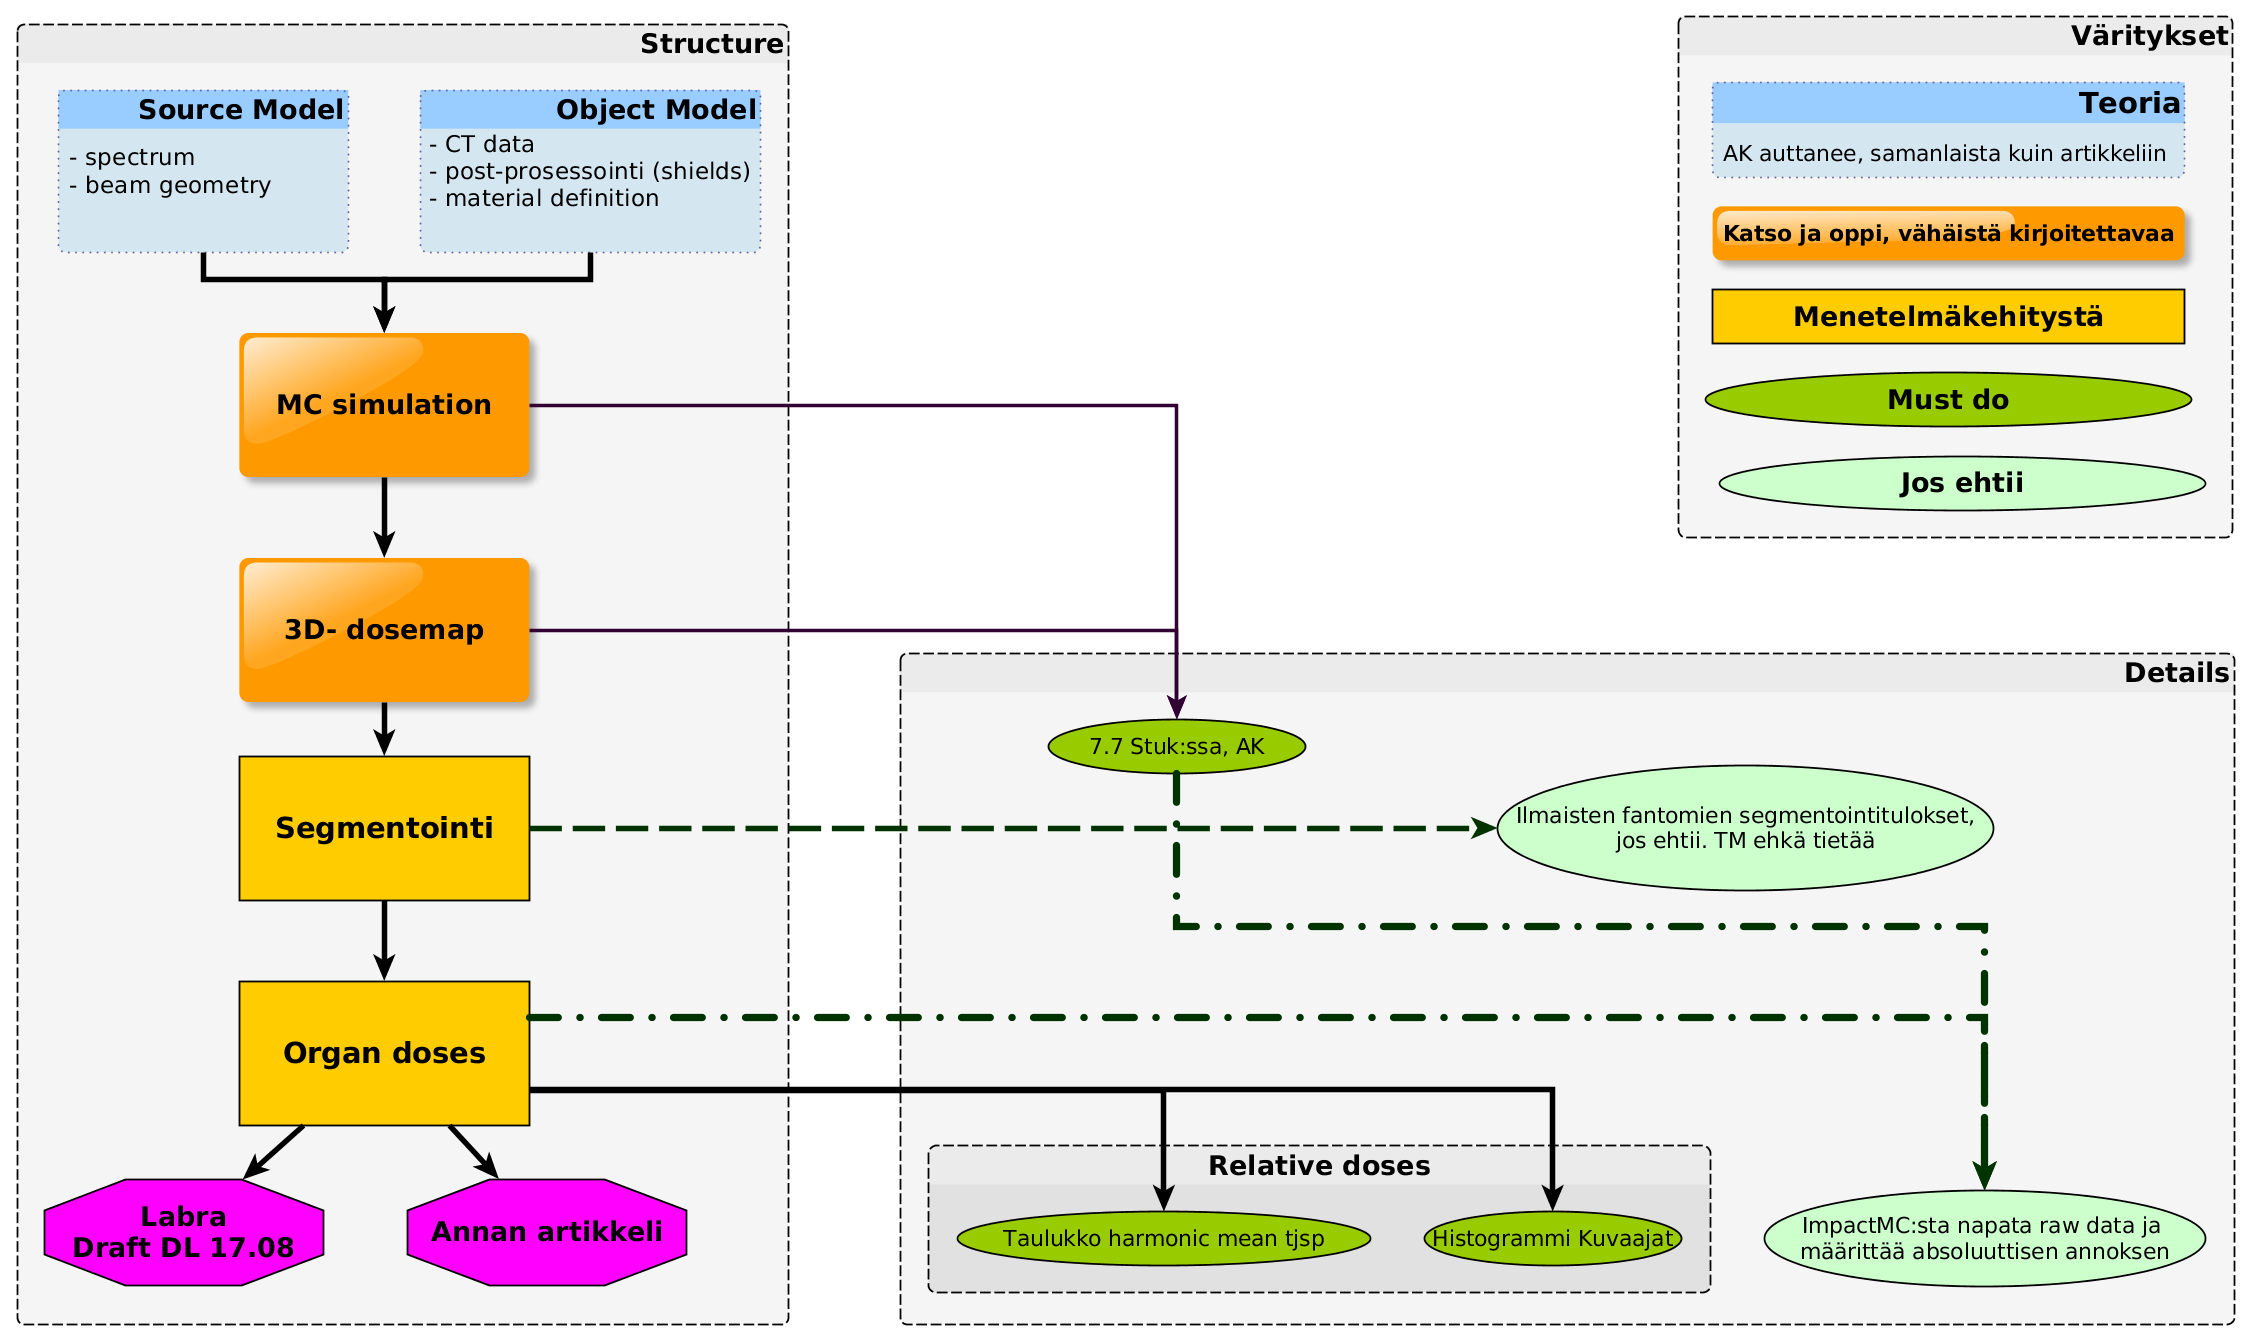
\includegraphics[width=\linewidth]{TT_SyvLabraSofiev_Plan}
\caption{Plan graph}
\label{fig:TT_SyvLabraSofiev_Plan}
\end{figure*}

\subsection*{No Shield relative / absolute doses}
\textit{\textbf{Listaa tänne kaikki kuvat suurkokoisina}}

Fig.\ref{fig:TT_SyvLabraSofiev_Plan}.
\begin{figure*}[ht]\centering
%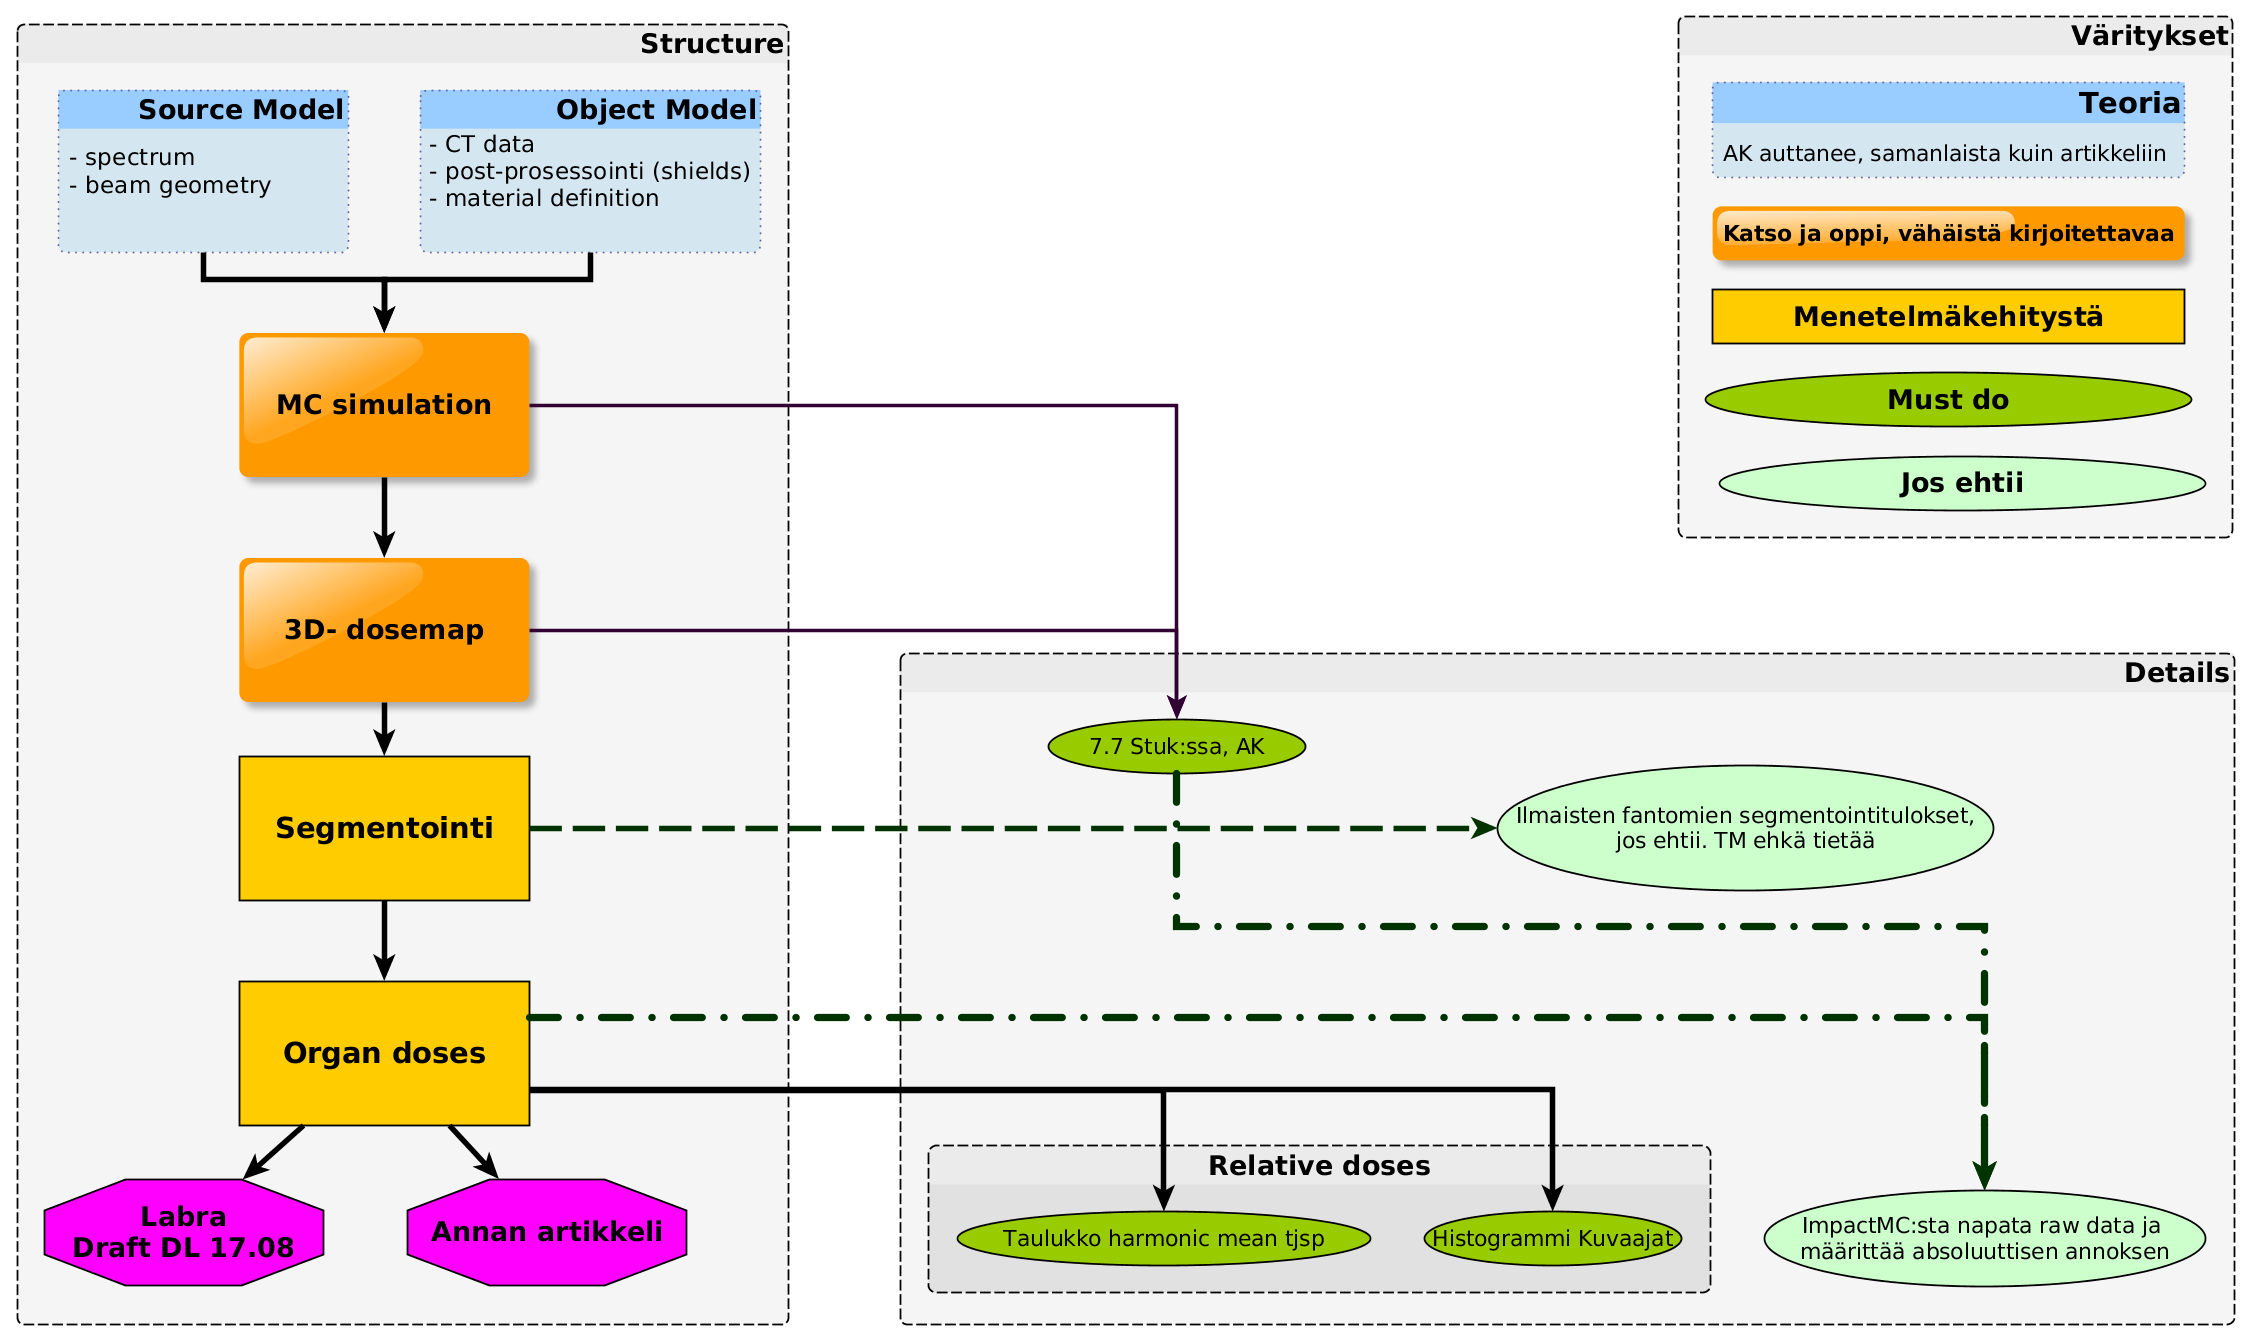
\includegraphics[width=\linewidth]{TT_SyvLabraSofiev_Plan}
\missingfigure{No shield image, histogram of ***}

\caption{Plan graph}
\label{fig:TT_SyvLabraSofiev_Plan}
\end{figure*}



%----------------------------------------------------------------------------------------
%	REFERENCE LIST
%----------------------------------------------------------------------------------------
\phantomsection
\bibliographystyle{unsrt}
\bibliography{sample}

%----------------------------------------------------------------------------------------

\end{document}